\documentclass[10pt,a4paper,openany]{memoir}
\makeatletter
\createmark{chapter}{both}{shownumber}{\@chapapp\ }{. \ }
\makeatother
\makeheadrule{headings}{\textwidth}{0.3pt}
\makeevenfoot{headings}{\thepage}{}{}
\makeoddfoot{headings}{}{}{\thepage}
\makeoddhead{headings}{}{}{\rightmark}
\makeevenhead{headings}{\leftmark}{}{}
\makeevenfoot{plain}{\thepage}{}{}
\makeoddfoot{plain}{}{}{\thepage}
\clearmark{section}
\usepackage{overcite}
\usepackage[utf8]{inputenc}
\usepackage{amsmath}
\usepackage{amsfonts}
\usepackage{booktabs}
\usepackage{longtable}
\usepackage{amssymb}
\usepackage{graphicx}
\usepackage{listings}
\usepackage{lmodern}
\usepackage{gensymb}
\usepackage{hyperref}
\usepackage{lscape}
\numberwithin{equation}{section}
\def\chapterautorefname{Chapter}
\def\sectionautorefname{Section}
\def\subsectionautorefname{Section}
\def\pageautorefname{p.}
\DeclareMathOperator{\sign}{sign}
\renewcommand*{\thefootnote}{\fnsymbol{footnote}}
\newcommand{\under}{\_}
\newcommand{\rsub}[1]{\mathbf{r}_{#1}}
\newcommand{\fsub}[1]{\mathbf{f}_{#1}}
\newcommand{\ssub}[1]{\mathbf{s}_{#1}}
\newcommand{\revyan}[1]{{\color{red}{[#1]}}}
\newcommand{\profileropt}[0]{\texttt{profilerOpt}}
\newcommand{\profilergen}[0]{\texttt{profilerGen}}
\newcommand{\profilertools}[0]{\texttt{profilerTools}}
\usepackage[left=.75in,right=.75in,top=.5in,bottom=.75in]{geometry}
\usepackage{color}

\definecolor{mygreen}{rgb}{0,0.6,0}
\definecolor{mygray}{rgb}{0.85,0.85,0.85}
\definecolor{mymauve}{rgb}{0.58,0,0.82}

% \setlength{\droptitle}{50pt}
\renewcommand{\maketitlehooka}{%
  \vfill\hrulefill}
\renewcommand{\maketitlehookb}{%
  \hrulefill\par \hfill \textit{Corresponding to Version 1.0}}
\renewcommand{\maketitlehookc}{%
  \vfill}
\title{\Huge\texttt{profilerTools} \\ User Manual}
\author{{\huge MSSM Group} \\ Maintained by Yan M. H. Gonçalves}
\date{\footnotesize\textcopyright 2020--: \hspace{5ex}
  MSSM Group, Laboratório de Modelagem Molecular,\\
  \hspace{16ex} Instituto de Química, Universidade Federal do Rio de Janeiro}
  
\lstdefinelanguage{gromacs}{morecomment=[l]{;}}
\lstset{
  backgroundcolor=\color{mygray},   % choose the background color; you must add \usepackage{color} or \usepackage{xcolor}; should come as last argument
  basicstyle=\footnotesize\ttfamily,        % the size of the fonts that are used for the code
  breakatwhitespace=false,         % sets if automatic breaks should only happen at whitespace
  belowskip=-4pt,
    aboveskip=-4pt,
  breaklines=true,                 % sets automatic line breaking
  captionpos=b,                    % sets the caption-position to bottom
  commentstyle=\color{mygreen},    % comment style
  deletekeywords={...},            % if you want to delete keywords from the given language
  escapeinside={\%*}{*)},          % if you want to add LaTeX within your code
  extendedchars=true,              % lets you use non-ASCII characters; for 8-bits encodings only, does not work with UTF-8
  firstnumber=01,                % start line enumeration with line 1000
  frame=single,	                   % adds a frame around the code
  keepspaces=true,                 % keeps spaces in text, useful for keeping indentation of code (possibly needs columns=flexible)
%  keywordstyle=\color{blue},       % keyword style
  language=Bash,                 % the language of the code
  morekeywords={*,...},            % if you want to add more keywords to the set
  numbers=none,                    % where to put the line-numbers; possible values are (none, left, right)
  numbersep=5pt,                   % how far the line-numbers are from the code
  numberstyle=\tiny\color{mygray}, % the style that is used for the line-numbers
  rulecolor=\color{white},         % if not set, the frame-color may be changed on line-breaks within not-black text (e.g. comments (green here))
  showspaces=false,                % show spaces everywhere adding particular underscores; it overrides 'showstringspaces'
  showstringspaces=false,          % underline spaces within strings only
  showtabs=false,                  % show tabs within strings adding particular underscores
  stepnumber=1,                    % the step between two line-numbers. If it's 1, each line will be numbered
  stringstyle=\color{mymauve},     % string literal style
  tabsize=4,	                   % sets default tabsize to 2 spaces
  columns=fullflexible,  
  title=\lstname                   % show the filename of files included with \lstinputlisting; also try caption instead of title
}

\lstdefinestyle{ascii-tree}{
    literate={├}{|}1 {─}{--}1 {└}{+}1 
  }
  \begin{document}
  \maketitle
  \thispagestyle{empty}

  \clearpage
  \frontmatter
  \nouppercaseheads
  \addtolength{\headheight}{2ex}
  \addtolength{\headsep}{-2ex}

  \section{Citation Information}

  % If the \profilertools{} suite was helpful in achieving your results,
  % we kindly ask you to cite the following paper:

  % \begin{quote}
  %   Long title of the paper, with many things. Many details of the
  %   journal, such as name and pages. Possibly also a DOI: xxxxxxx.
  % \end{quote}

  % \noindent If you wish to cite this manual, please refer to it as

  % \begin{quote}
  %   Gonçalves, Y.~M.~H. \textit{profilerTools: User Manual
  %   (v1.0)}. \url{https://github.com/mssm-labmmol/profiler} (2020).
  % \end{quote}

  In the absence of a scientific publication, we kindly ask you to
  cite this manual if the \profilertools{} suite was helpful in
  achieving your results, referring to it as

  \begin{quote}
    Gonçalves, Y.~M.~H. and the MSSM Group. \textit{profilerTools: User Manual
      (Version 1.0)}.\\
    \url{https://github.com/mssm-labmmol/profiler}
    (2020).
  \end{quote}

  \section{License}

  \profilertools{} is released under the MIT License. For more
  information, check the LICENSE file supplied with the source code or
  consult \autoref{appendix:MIT-license}

  \section{Contact}

  For bug reports or other software-related questions, send an e-mail
  to \url{yanmarques@gmail.com}.  More information about our research
  group can be found on the webpage
  \url{https://labmmol.iq.ufrj.br/mssm}.

\tableofcontents

  \mainmatter

\newcommand*{\profi}{\texttt{profilerOpt}}

\chapter{Molecular Mechanics}
\label{chap:mm}

All molecular-mechanics calculations are performed using custom code which depends only on standard Python libraries and \texttt{numpy}.
In this chapter, we report all functional forms supported for the
calculation of molecular-mechanics energies and forces.
The following notation and definitions will be used for mathematical and physical quantities whenever convenient:

\begin{itemize}
\item[---] $\mathbf{u} \cdot \mathbf{v}$ \par \hspace{10ex} Dot product of vectors $\mathbf{u}$ and $\mathbf{v}$.
\item[---] $\mathbf{u} \times \mathbf{v}$ \par \hspace{10ex} Cross product of vectors $\mathbf{u}$ and $\mathbf{v}$.
\item[---] $\mathbf{r}_i$ \par \hspace{10ex} Position of particle $i$.
\item[---] $\mathbf{r}_{ij} = \mathbf{r}_i - \mathbf{r}_j$ \par \hspace{10ex} Displacement from particle $j$ to particle $i$.
\item[---] $r_{ij} = \sqrt{\mathbf{r}_{ij} \cdot \mathbf{r}_{ij}}$ \par \hspace{10ex} Distance between particle $i$ and particle $j$.
\item [---] $\theta_{ijk} = \arccos{\frac{\mathbf{r}_{ij} \cdot \mathbf{r}_{kj}}{r_{ij}r_{kj}}}$  \par \hspace{10ex} Angle involving particles $i$, $j$ and $k$.
  \item [---] $\phi_{ijkl} = \sign{(\rsub{ij} \cdot \rsub{nk})} \arccos{\left( \frac{\rsub{mj} \cdot \rsub{nk}}{r_{mj}r_{nk}} \right)}$, with $\rsub{mj} = \rsub{ij}\times\rsub{kj}$ and $\rsub{nk} = \rsub{kj}\times\rsub{kl}$
     \par \hspace{10ex} Dihedral-angle involving particles $i$, $j$, $k$ and $l$.
   \end{itemize}

\section{Bond stretching}
\label{sec:bond-terms}

The following functional forms are supported for the calculation of
the energies and forces associated with a bond-stretching degree of freedom:\cite{GROMOS-doc,GROMACS-doc}

\begin{itemize}
\item [---] \textit{Harmonic}
  \par
  Potential energy form:
  \begin{align}
    \label{eq:harmonic-bond-energy}
    V(r_{ij}; k_b^h, b_0) & = \frac{1}{2} \ k_b^h (r_{ij} - b_0)^2 \quad , \\ \nonumber
    \frac{\partial V(r_{ij}; k_b^h, b_0)}{\partial r_{ij}} & = \ k_b^h (r_{ij} - b_0) \quad ,
  \end{align}
  
\item [---] \textit{Quartic}
  \par
  Potential energy form:
  \begin{align}
    \label{eq:quartic-bond-energy}
    V(r_{ij}; k_b^q, b_0) & = \frac{1}{4} \ k_b^q (r_{ij}^2 - b_0^2)^2 \quad , \\ \nonumber
    \frac{\partial V(r_{ij}; k_b^q, b_0)}{\partial r_{ij}} & = r_{ij} k_b^q (r_{ij}^2 - b_0^2) \quad ,
  \end{align}

\end{itemize}

\noindent
where $V(r_{ij})$ is the potential energy term for the bond between particles $i$ and $j$.

\section{Bond-angle stretching}
\label{sec:angle-terms}

The following functional forms are supported for the calculation of
the energies and forces associated with a bond-angle stretching degree of freedom:\cite{GROMOS-doc,GROMACS-doc}

\begin{itemize}
\item [---] \textit{Harmonic}
  \par
  Potential energy form:
  \begin{align}
    \label{eq:harmonic-angle-energy}
    V(\theta_{ijk}; k_a^h, \theta_0) & = \frac{1}{2} \ k_a^h (\theta_{ijk} - \theta_0)^2 \quad , \\ \nonumber
    \frac{\partial V(\theta_{ijk}; k_a^h, \theta_0)}{\theta_{ijk}} & = k_a^h (\theta_{ijk} - \theta_0) \quad ,
  \end{align}
  
\item [---] \textit{Cosine-harmonic}
  \par
  Potential energy form:
  \begin{align}
    \label{eq:cosine-angle-energy}
    V(\theta_{ijk}; k_a^c, \theta_0) & = \frac{1}{2} \ k_a^c (\cos{\theta_{ijk}} - \cos\theta_0)^2 \quad , \\ \nonumber
    \frac{\partial V(\theta_{ijk}; k_a^c, \theta_0)}{\theta_{ijk}} & = -k_a^c \sin{\theta_{ijk}}(\cos{\theta_{ijk}} - \cos\theta_0) \quad ,
  \end{align}

\item [---] \textit{Urey-Bradley}
  \par
  Potential energy form:
  \begin{align}
    \label{eq:ub-angle-energy}
    V(\theta_{ijk},r_{ik}; k_a^{ub}, \theta^{ub}_0,k_{13}^{ub},b_{13}^{ub}) & = \frac{1}{2} \ k_a^{ub} (\theta_{ijk} - \theta_0)^2 + \frac{1}{2}  \ k_{13}^{ub} (r_{ik} - b_{13}^{ub})^2 \quad , \\ \nonumber
    \frac{\partial V(\theta_{ijk},r_{ik}; k_a^{ub}, \theta^{ub}_0,k_{13}^{ub},b_{13}^{ub})}{\partial \theta_{ijk}} & = k_a^{ub} (\theta_{ijk} - \theta_0) \quad , \\ \nonumber
    \frac{\partial V(\theta_{ijk},r_{ik}; k_a^{ub}, \theta^{ub}_0,k_{13}^{ub},b_{13}^{ub})}{\partial r_{ik}}  & = k_{13}^{ub} (r_{ik} - b_{13}^{ub}) \quad ,
  \end{align}

\end{itemize}  
\noindent
where $V(\theta_{ijk},[r_{ik}])$ is the potential energy term for the angle involving particles $i$, $j$ and $k$.
Note that the Urey-Bradley form introduces dependence on an additional degree of freedom, the distance $r_{ik}$, which is treated as a harmonic bond between particles $i$ and $k$.

\section{Proper dihedral-angle torsion}
\label{sec:proper-terms}

The following functional forms are supported for the calculation of
the energies and forces associated with a proper dihedral-angle
torsion degree of freedom:\cite{GROMOS-doc,GROMACS-doc}

\begin{itemize}
\item [---] \textit{Standard periodic}
  \par
  Potential energy form:
  \begin{align}
    \label{eq:proper-standard-energy}
    V(\phi_{ijkl} ; \{k_{d,m}^s, \phi_{0,m}\}_{m=1..6}) & = \sum_{m=1}^{N_T} k_{d,m}^s\ (1 + \cos{\phi_{0,m}} \cos{m \phi_{ijkl}})\quad , \\ \nonumber
    \frac{\partial V(\phi_{ijkl} ; \{k_{d,m}^s, \phi_{0,m}\}_{m=1..6})}{\partial \phi_{ijkl}} & = -\sum_{m=1}^{N_T} m k_{d,m}^s \cos{\phi_{0,m}} \sin{m \phi_{ijkl}}\quad ,
  \end{align}
  with $\phi_{0,m}=0,\pi$.
  
\item [---]\textit{Ryckaert-Bellemans}
  \par
  Potential energy form:
  \begin{align}
    \label{eq:proper-rb-energy}
    V(\phi_{ijkl} ; \{c_m\}_{m=0..5}) & = \sum_{m=0}^{5} c_m \cos^m{(\phi_{ijkl}-\pi)} \quad , \\ \nonumber
    \frac{\partial V(\phi_{ijkl} ; \{c_m\}_{m=0..5})}{\partial \phi_{ijkl}} & = \sum_{m=1}^{5} mc_m \sin{\phi_{ijkl}} \cos^{m-1}{(\phi_{ijkl}-\pi)} \quad , 
  \end{align}

\item [---]\textit{Fourier}
  \par
  Potential energy form:
   \begin{align}
    \label{eq:proper-fourier-energy}
     V(\phi_{ijkl} ; \{f_m\}_{m=1..4}) & = \frac{1}{2} \sum_{m=1}^{4} f_m \left[1 + (-1)^{m+1}\cos m\phi_{ijkl}\right] \quad , \\ \nonumber
     \frac{\partial V(\phi_{ijkl} ; \{f_m\}_{m=1..4})}{\partial \phi_{ijkl}} & = \frac{1}{2} \sum_{m=1}^{4} m f_m (-1)^{m}\sin m\phi_{ijkl} \quad ,
   \end{align}
   
   Internally, this potential is computed as a Ryckaert-Bellemans potential with
   \begin{align*}
     c_0 & = f_2 + \frac{1}{2} (f_1 + f_3)\\
     c_1 & = \frac{1}{2} (-f_1 + 3f_3)\\
     c_2 & = -f_2 + 4f_4\\
     c_3 & = -2 f_3\\
     c_4 & = -4 f_4\\
     c_5 & = 0
   \end{align*}

\item [---]\textit{Harmonic restraint}
  \par
  Potential energy form:
  \begin{align}
  \label{eq:proper-restraint-energy}
  V(\phi_{ijkl}; k_d^r, \phi_0) & = \frac{1}{2} k_d^r (\phi_{ijkl} - \phi_0)^2 \quad , \\ \nonumber
  \frac{\partial V(\phi_{ijkl}; k_d^r, \phi_0)}{\partial \phi_{ijkl}} & = k_d^r (\phi_{ijkl} - \phi_0) \quad , 
\end{align}
\end{itemize}
where $V(\phi_{ijkl})$ is the potential energy term for the proper dihedral-angle involving particles $i$, $j$, $k$ and $l$.

\section{Improper dihedral-angle bending}
\label{sec:improper-terms}

The following functional forms are supported for the calculation of
the energies and forces associated with an improper dihedral-angle
bending degree of freedom:\cite{GROMOS-doc,GROMACS-doc}

\begin{itemize}
\item[---] \textit{Harmonic}
  \par
  Potential energy form:  
\begin{align}
  \label{eq:improper-harmonic-energy}
  V(\phi_{ijkl}; k_i^h, \phi_0) & =  \frac{1}{2} k_i^h (\phi_{ijkl} - \phi_0)^2 \quad , \\ \nonumber
  \frac{\partial V(\phi_{ijkl}; k_i^h, \phi_0)}{\phi_{ijkl}} & = k_i^h (\phi_{ijkl} - \phi_0) \quad ,
\end{align}
\item [---] \textit{Periodic}
  \par
  Potential energy form:
  \begin{align}
    \label{eq:improper-periodic-energy}
    V(\phi_{ijkl} ; k_{i}^p, \phi_{0}, m) & = k_{i}^p\ (1 + \cos{\phi_{0}} \cos{m \phi_{ijkl}})\quad , \\ \nonumber
    \frac{\partial V(\phi_{ijkl} ; k_{i}^p, \phi_{0}, m)}{\partial \phi_{ijkl}} & = -m k_{i}^p \cos{\phi_{0}} \sin{m \phi_{ijkl}}\quad ,
  \end{align}
  with $\phi_{0}=0,\pi$.
 \end{itemize}
 where $V(\phi_{ijkl})$ is the potential energy term for the improper dihedral-angle involving particles $i$, $j$, $k$ and $l$.

\section{Nonbonded interactions}
\label{sec:nonbonded}

\subsection{Standard interactions}
\label{sec:standard-lj-interactions}

The nonbonded interactions are calculated for every pair of
non-excluded particles, without applying any type of cutoff-based
truncation.  The electrostatic and van der Waals interactions are
calculated based on the following functional forms, respectively:\cite{GROMOS-doc,GROMACS-doc}

\begin{itemize}
\item[---] \textit{Coulomb}
  \begin{align}
  \label{eq:coulomb-term}
    V(r_{ij};q_i,q_j) & = \frac{q_i q_j}{4\pi\epsilon_0 r_{ij}} \quad , \\ \nonumber
    \frac{\partial V(r_{ij};q_i,q_j)}{\partial r_{ij}} & = -\frac{q_i q_j}{4 \pi \epsilon_0 r_{ij}^2} \quad ,
\end{align}
\item[---] \textit{Lennard-Jones}
    \begin{align}
  \label{eq:lj-term}
      V(r_{ij};C_{6,ij},C_{12,ij}) & = \frac{C_{12,ij}}{r_{ij}^{12}} - \frac{C_{6,ij}}{r_{ij}^6} \quad , \\ \nonumber
      \frac{\partial V(r_{ij};C_{6,ij},C_{12,ij})}{r_{ij}} & = -\frac{6}{r_{ij}^8}\left(\frac{2C_{12,ij}}{r_{ij}^{6}} - C_{6,ij} \right) \quad ,
\end{align}
\end{itemize}
where the interaction between particles $i$ and $j$ is considered.

When the pair-specific $C_{12,ij}$ and
$C_{6,ij}$ Lennard-Jones parameters are not explicitly defined,
they are obtained from atomic
counterparts, using one of the following mixing rules:
\begin{itemize}
\item [---] \textit{Geometric}
  \begin{equation}
    \label{eq:geometric-mix}
    C_{6,ij} = \sqrt{C_{6,i}C_{6,j}} \quad , \quad C_{12,ij} = \sqrt{C_{12,i}C_{12,j}}
  \end{equation}
\item [---]\textit{Lorentz-Berthelot}
  \begin{align}
    \label{eq:lorentz-mix}
    C_{6,ij} &= \frac{C_{6,i}C_{6,j}}{2^6 \sqrt{C_{12,i}C_{12,j}}}\left[\left(\frac{C_{12,i}}{C_{6,i}}\right)^{1/6} + \left(\frac{C_{12,j}}{C_{6,j}}\right)^{1/6} \right]^6  \\ \nonumber
    C_{12,ij} &= \frac{C_{6,i}C_{6,j}}{2^{12} \sqrt{C_{12,i}C_{12,j}}}\left[\left(\frac{C_{12,i}}{C_{6,i}}\right)^{1/6} + \left(\frac{C_{12,j}}{C_{6,j}}\right)^{1/6} \right]^{12} \quad .
  \end{align}
\end{itemize}

Internally, the $C_6$-$C_{12}$ representation of the Lennard-Jones
potential is always used.  However, some force fields are
traditionally specified in terms of the $\sigma$-$\epsilon$
representation of the Lennard-Jones potential:
\begin{itemize}
  \item [---] \textit{Lennard-Jones} ($\sigma$-$\epsilon$)
\begin{equation}
  \label{eq:lj-sigma-epsilon-term}
  V(r_{ij}; \sigma_{ij}, \epsilon_{ij}) = 4\epsilon_{ij}\left[ \left(\frac{\sigma_{ij}}{r_{ij}}\right)^{6} - \left(\frac{\sigma_{ij}}{r_{ij}}\right)^{12}   \right] \ , \ \sigma_{ij} = (C_{12,ij}/C_{6,ij})^{1/6} \ , \ \epsilon_{ij} = C_{6,ij}^2/4C_{12,ij}
\end{equation}
\end{itemize}
with corresponding mixing rules
\begin{itemize}
\item [---] \textit{Geometric}
  \begin{equation}
    \label{eq:geometric-mix-sigma-epsilon}
  \sigma_{ij} = \sqrt{\sigma_i \sigma_j} \quad , \quad \epsilon_{ij} = \sqrt{\epsilon_i \epsilon_j}
  \end{equation}
\item [---]\textit{Lorentz-Berthelot}
  \begin{align}
    \label{eq:lorentz-mix-sigma-epsilon}
  \sigma_{ij} = \frac{1}{2}(\sigma_i + \sigma_j) \quad , \quad \epsilon_{ij} = \sqrt{\epsilon_i \epsilon_j} \quad .
  \end{align}
\end{itemize}

\subsection{1--4 interactions}
\label{sec:1-4-interactions}

The interactions of pairs of particles that are identified as sharing
a third-neighbor relationship (1--4 interactions) are treated in a
different manner. First, all 1--4 Coulomb interactions are scaled down from
their standard values by a common factor $f_{QQ}$ as
\begin{equation}
  \label{eq:fudge-QQ}
    V(r_{ij};q_i,q_j) = f_{QQ}\ \frac{q_i q_j}{4\pi\epsilon_0 r_{ij}} \quad , \quad 0 \leq f_{QQ} \leq 1\ .
\end{equation}
For the 1--4 Lennard-Jones interactions, the options listed below are available.
The first is more common and establishes a simple rule for computing 1--4 Lennard-Jones parameters based on the standard Lennard-Jones parameters.
The second is more uncommon (but is used \textit{e.g.} in GROMOS force fields) and relies on defining additional atomic Lennard-Jones parameters to use exclusively with 1--4 interactions. 
\begin{itemize}
\item [---] Scale down the standard atomic parameters by a common factor $f_{LJ}$, obtaining 1--4 atomic parameters $CS_{6} = f_{LJ}C_{6}$ and $CS_{12} = f_{LJ}C_{12}$. After that, proceed as usual, obtaining the 1--4 pair parameters $CS_{12,ij}$ and $CS_{6,ij}$ \textit{via} mixing rule and computing the scaled-down potential energy:
  \begin{equation}
    \label{eq:fudge-LJ}
    V(r_{ij};C_{6,ij},C_{12,ij}) =   \frac{CS_{12,ij}}{r_{ij}^{12}} - \frac{CS_{6,ij}}{r_{ij}^6} = f_{LJ} \left( \frac{C_{12,ij}}{r_{ij}^{12}} - \frac{C_{6,ij}}{r_{ij}^6} \right) \quad , \quad 0 \leq f_{LJ} \leq 1
  \end{equation}
% \item [---] Explicitly specify 1--4 values $CS_{12,ij}$ and $CS_{6,ij}$ for the pair interaction:
%   \begin{equation}
%     \label{eq:explicit-LJ}
%       V(r_{ij};CS_{6,ij},CS_{12,ij}) = \frac{CS_{12,ij}}{r_{ij}^{12}} - \frac{CS_{6,ij}}{r_{ij}^6} \right)
%   \end{equation}
\item [---] Instead of using a fixed factor $f_{LJ}$ to modify the atomic parameters, specify an additional arbitrary set of atomic parameters $CS_6$ and $CS_{12}$ which are exclusive to 1--4 interactions. The 1--4 pair parameters $CS_{12,ij}$ and $CS_{6,ij}$ are then obtained \textit{via} mixing rule, resulting in a pair-specific scaled-down potential energy
    \begin{equation}
    \label{eq:atomic-LJ}
    V(r_{ij};CS_{6,ij},CS_{12,ij}) =  \frac{CS_{12,ij}}{r_{ij}^{12}} - \frac{CS_{6,ij}}{r_{ij}^6} 
  \end{equation}
\end{itemize}

\section{Forces}
\label{sec:forces}

The atomic forces due to the potential energy terms reported above are
obtained by computing the analytical derivatives of the corresponding
expressions with respect to the atomic positions involved in the
degree of freedom.  In general,

\begin{itemize}
  \item[---]\textit{Bond terms and nonbonded terms}
\begin{equation}
  \label{eq:bond-forces}
  \mathbf{f}_\alpha = -\frac{\partial V(r_{ij})}{\partial r_{ij}}\ \nabla_{\mathbf{r}_{\alpha}} r_{ij}\quad , \quad \alpha = i,j \quad ,
\end{equation}
  \item[---]\textit{Angle terms}
\begin{equation}
  \label{eq:angle-forces}
  \mathbf{f}_\alpha = -\frac{\partial V(\theta_{ijk})}{\partial \theta_{ijk}}\ \nabla_{\mathbf{r}_{\alpha}} \theta_{ijk}\quad , \quad \alpha = i,j,k \quad ,
\end{equation}
  \item[---]\textit{Dihedral terms}
\begin{equation}
  \label{eq:dihedral-forces}
  \mathbf{f}_\alpha = -\frac{\partial V(\phi_{ijkl})}{\partial \phi_{ijkl}}\ \nabla_{\mathbf{r}_{\alpha}} \phi_{ijkl}\quad , \quad \alpha = i,j,k,l \quad ,
\end{equation}
\end{itemize}
where $\mathbf{f}_\alpha$ is the force acting on particle $\alpha$ and
$\nabla_{\mathbf{r}_\alpha}$ denotes the gradient with respect to the
position of particle $\alpha$. Each expression above is the product of
a straightforward uni-dimensional derivative involving the potential
expression with a more complicated ``geometrical'' derivative. The
former terms are reported in the Sections above for each functional
form. The latter terms are common to all interactions and are listed
below:

\begin{itemize}
  \item [---]\textit{Bond terms and nonbonded terms}
  \begin{align}
  \label{eq:distance-gradient}
  \nabla_{\mathbf{r}_i}r_{ij} & = +\frac{\mathbf{r}_{ij}}{r_{ij}} \\ \nonumber
  \nabla_{\mathbf{r}_j}r_{ij} & = -\frac{\mathbf{r}_{ij}}{r_{ij}}
  \end{align}
  \item[---]\textit{Angle terms}
\begin{align}
  \label{eq:angle-gradient}
  \nabla_{\mathbf{r}_i}\theta_{ijk} & = +\frac{1}{r_{ij}}\left( \frac{\rsub{kj}}{r_{kj}} - \frac{\rsub{ij}}{r_{ij}} \cos \theta_{ijk} \right) \\ \nonumber
  \nabla_{\mathbf{r}_j}\theta_{ijk} & = -\nabla_{\mathbf{r}_i}\theta_{ijk}-\nabla_{\mathbf{r}_k}\theta_{ijk} \\ \nonumber
  \nabla_{\mathbf{r}_k}\theta_{ijk} & = +\frac{1}{r_{kj}}\left( \frac{\rsub{ij}}{r_{ij}} - \frac{\rsub{kj}}{r_{kj}} \cos \theta_{ijk} \right)
\end{align}
\item [---]\textit{Dihedral terms}
  \begin{align}
    \label{eq:dihedral-gradient}
    \nabla_{\mathbf{r}_i}\phi_{ijkl} & = +\frac{r_{kj}}{r_{mj}^2}\rsub{mj} \\ \nonumber
    \nabla_{\mathbf{r}_j}\phi_{ijkl} & = +\left[\frac{\rsub{ij}\cdot\rsub{kj}}{r_{kj}^2}- 1\right]\nabla_{\rsub{i}}\phi_{ijkl} - \frac{\rsub{kl}\cdot\rsub{kj}}{r_{kj}^2}\nabla_{\rsub{l}}\phi_{ijkl}\\ \nonumber
    \nabla_{\mathbf{r}_k}\phi_{ijkl} & = -\nabla_{\rsub{i}}\phi_{ijkl} - \nabla_{\rsub{j}}\phi_{ijkl} - \nabla_{\rsub{l}}\phi_{ijkl}\\ \nonumber
    \nabla_{\mathbf{r}_l}\phi_{ijkl} & = +\frac{r_{kj}}{r_{nk}^2}\rsub{nk}  \quad ,
  \end{align}
  where
  \begin{align*}
    \rsub{mj} = \rsub{ij}\times\rsub{kj}\ ,\ \rsub{nk} = \rsub{kj}\times\rsub{kl}\quad .
  \end{align*}
\end{itemize}

\section{Choice of functional forms}
\label{sec:choice-of-functional-forms}

The functional forms used for each interaction term are selected in
the input STP file via type codes. Likewise, the Lennard-Jones
potential representation, mixing rule and 1--4 details are specified
in this same file. For more information, read the STP file format
section on \autoref{chap:file-formats}.

\section{Limitations}
\label{sec:limitations}

\begin{itemize}
\item[---] Periodic boundary conditions are currently not taken into
  account. Please make sure your systems fit entirely within the
  central simulation box to avoid any problems.
\item[---] The nonbonded interactions are computed explicitly
  regardless of the distance between the interacting particles. No
  other scheme for computing the nonbonded interactions is currently
  supported.
\item[---] Only one functional form is accepted for each type of
  bonded interaction. The only exception is for proper dihedral
  restraints, which can be defined along with any other form of proper
  dihedral term. 
\end{itemize}

\chapter{Energy Minimization}
\label{chap:minim}

In this chapter, we briefly describe the energy minimization algorithms implemented in the program, namely
\textit{steepest-descents} and
\textit{conjugate-gradients}.
Both implementations are based on the descriptions supplied in the GROMOS user manual\cite{GROMOS-doc}.
The following notation will be used:

\begin{itemize}
\item [---] $\mathbf{r}(t_n) = (\rsub{1}(t_n),\rsub{2}(t_n)\ldots\rsub{N}(t_n))$
  \par
  \hspace{10ex}
  Configuration of the system of $N$ particles at the $n$-th step of the algorithm.
\item [---] $\mathbf{f}(t_n) = (\fsub{1}(t_n),\fsub{2}(t_n)\ldots\fsub{N}(t_n))$
  \par
  \hspace{10ex}
  Configuration of the forces of the system of $N$ particles at the $n$-th step of the algorithm.
\end{itemize}

\section{Steepest-descents}
\label{sec:steep}

In the steepest-descents energy minimization algorithm, one successively updates the configuration by moving along the direction of the gradient of the potential energy over the configurational space.
The $n$-th step of the steepest-descents energy minimization algorithm is as follows: 
\begin{enumerate}
\item Calculate $\mathbf{f}(t_n)$ from the configuration $\mathbf{r}(t_n)$.
\item Compute the next configuration from
  \begin{equation}
    \label{eq:em-steep}
  \mathbf{r}(t_{n+1}) = \mathbf{r}(t_n) + \frac{\Delta x(t_n)}{\sqrt{\sum_{i=1}^N \fsub{i}(t_n)\cdot\fsub{i}(t_n)}}\ \mathbf{f}(t_n) \quad .
  \end{equation}
\end{enumerate}

The initial value of the step size $\Delta x(t_n)$ is specified in the input variable DX0.
If the energy decreases in a given step $n$, $\Delta x(t_{n+1}) = \min{\{1.2\cdot\Delta x(t_{n}),\ \text{DXM}\}}$, where DXM is an input variable.
If the energy increases, $\Delta x(t_{n+1}) = 0.5\cdot\Delta x(t_{n})$.
The algorithm is terminated if the number of steps reaches the value specified in the input variable NMAX or if the energy difference between successive steps is less than the one specified in the input variable DELE.

For more information on the input variables above, see \autoref{chap:file-formats}.

\section{Conjugate-gradients}
\label{sec:conjugate-gradients}

In the conjugate-gradients energy minimization algorithm, one does not move strictly along the gradient of the potential energy over the configurational space.
Instead, a search direction
\begin{equation}
  \label{eq:em-cg-search}
   \mathbf{s}(t_n) = \mathbf{f}(t_n) + \mathbf{s}(t_{n-1}) \frac{\sum_{i=1}^{N}\fsub{i}(t_n)\cdot\fsub{i}(t_{n-1})}{\sum_{i=1}^{N}\fsub{i}(t_{n-1})\cdot\fsub{i}(t_{n-1})} 
\end{equation}
is defined for each step, with $\mathbf{s}(t_0) = \mathbf{f}(t_0)$.
Let $V|_s(s;t_n) = V(\mathbf{r}(t_n) + s\cdot\mathbf{s}(t_n))$ be the restriction of the potential energy hypersurface to this search direction and
\begin{equation*}
  v(s;t_n) = - \sum_{i=1}^N \mathbf{f}_i(\mathbf{r}(t_n) + s\cdot\mathbf{s}(t_n)) \cdot \mathbf{s}_i(t_n) \quad , \quad \mathbf{s}(t_n) = (\mathbf{s}_1(t_n),\mathbf{s}_2(t_n) \ldots \mathbf{s}_N(t_n))
\end{equation*}
its derivative, where $\mathbf{f}_i(\mathbf{r}(t_n) + s\cdot\mathbf{s}(t_n))$ represents the forces on particle $i$ calculated for the configuration $\mathbf{r}(t_n) + s\cdot\mathbf{s}(t_n)$.
In terms of these real functions, the $n$-th step of the algorithm involves two substeps:
\begin{enumerate}
\item Find a small interval $I(t_n)=(a(t_n), b(t_n)]$ which is guaranteed to contain a local minimum of $V|s(s;t_n)$.
  \par
  The existence of a minimum in $I(t_n)$ is ensured by any of the following pairs of conditions:
  \begin{align*}
    \left\{
    \begin{array}{rcl}
      v(a(t_n)) & < &0 \\
     V|_s(b(t_n)) & \geq &V|_s(a(t_n))
      \end{array}\right.
               \quad\text{or}\quad
      \left\{
      \begin{array}{rcl}
        v(a(t_n)) & < & 0 \\
        v(b(t_n)) & \geq & 0
      \end{array}\right.
  \end{align*}
  The loop below is used to select adequate values for $a(t_n)$ and $b(t_n)$.
  
  Starting with $a_1(t_n) = 0$ and $b_1(t_n) = \Delta x\ (\sum_{i=1}^N \ssub{i}(t_n)\cdot\ssub{i}(t_n))^{-1/2}$, the $k$-th step is:
  \begin{enumerate}
  \item Compute the energies and forces for the configurations $\mathbf{r}(t_n) + a_k(t_n)\cdot\mathbf{s}(t_n)$ and $\mathbf{r}(t_n) + b_k(t_n)\cdot\mathbf{s}(t_n)$.
  \item Verify the terminating conditions above. If none of them are satisfied, proceed with $a_{k+1}(t_n) = b_{k}(t_n)$ and $b_{k+1}(t_n)=2b_k(t_n)$.
    Otherwise, $a(t_n) = a_k(t_n)$ and $b(t_n) = b_k(t_n)$.
  \end{enumerate}
  The step size $\Delta x$ is obtained from the input variable DX0.
  The loop is terminated with an error if, at any step, $b_{k+1}(t_n) \geq \text{DXM}$, where DXM is an input variable.
\item Obtain an estimate $s_{m}$ of the local minimum in $I(t_n)$ based on a cubic interpolation:
  \begin{align}
    \label{eq:em-cg-interp}
    s_m & = b - \frac{(b(t_n) - a(t_n))[W-Z+v(b(t_n))]}{v(b(t_n)) - v(a(t_n)) + 2W} \quad ,\\ \nonumber
    W & = \sqrt{Z^2-v(a(t_n))v(b(t_n))} \quad , \\ \nonumber
    Z & = \frac{3[V|_s(a(t_n)) - V|_s(b(t_n))]}{b(t_n) - a(t_n)} + v(a(t_n)) + v(b(t_n)) \quad .
  \end{align}
  If $V|_s(s_{m}) < V|_s(a(t_n))$ and $V|_s(s_{m}) < V|_s(b(t_n))$, accept the estimate as the local minimum and proceed with
  \begin{equation}
    \label{eq:em-cg-step}
    \mathbf{r}(t_{n+1}) = \mathbf{r}(t_n) + s_m \cdot \mathbf{s}(t_n) \quad ,
  \end{equation}
  updating the search direction with \autoref{eq:em-cg-search}.
  Otherwise, repeat the interpolation setting $b(t_n) = s_m$ (if $v(s_m) \geq 0$) or $a(t_n) = s_m$ (if $v(s_m) <0$).

\end{enumerate}

The algorithm is terminated if the number of steps reaches the value specified in the input variable NMAX or if the energy difference between successive steps is less than the value of the input variable DELE.
For more information on these input variables and others mentioned above, see \autoref{chap:file-formats}.

\chapter{Parameter Optimization}
\label{chap:ga}

In this chapter, we describe the structure of the parameter
optimization and how it is carried out in the context of a simple
genetic algorithm (GA) method implemented in the \profileropt{}
program. It is instructive to think of the optimization in terms of
three main parts:
\begin{enumerate}
\item The definition of the boundary conditions of the generation of
  trial parameters, \textit{i.e} setting the functional form of the
  torsional and Lennard-Jones terms involved in the GA
  (\autoref{sec:ga-bound}).

\item The application of these trial parameters in the modelling of
  the molecular systems of interest, whereby they acquire physical
  meaning as force-field parameters and their fitness can be assessed
  and used in the GA as feedback for the evolutionary process
  (\autoref{sec:ga-opt-control}, \autoref{sec:ga-tpes},
  \autoref{sec:ga-fitness-wei}).
  
\item The generation and evolution of trial parameters, controlled by
  the details of the GA (\textit{e.g.} crossover and mutation operators)
  and carried out in conformity with the items above
  (\autoref{sec:ga}).
\end{enumerate}

\section{Boundary Conditions}
\label{sec:ga-bound}

\profileropt{} admits a fairly flexible setup of boundary conditions
for the optimized parameters. In terms of the torsional parameters,
the user can select either a standard or Ryckaert-Bellemans functional
form, with customized summands. It is also possible to not optimize
torsional parameters at all. In terms of the Lennard-Jones parameters,
the user can opt on optimizing both attractive and repulsive
parameters, only one of them or none of them. For example, it is
possible to carry out a \profileropt{} run where only $CS_{12}$ and
odd-multiplicity terms of a standard proper dihedral form are taken
into account. The configuration of these boundary conditions is
performed in the INP input file, as described in
\autoref{sec:inp-parameter_optimization}.

\section{From Trial Parameters to Force-field Terms}
\label{sec:ga-opt-control}

In general, each molecular system contains several torsional and
Lennard-Jones degrees of freedom, and not all of them should be
modelled by the optimized parameters. In fact, for each system there
is a specific list of \textit{Optimized Dihedrals} (ODs) and
\textit{Optimized Pairs} (OPs) that convey the information of the
dihedral-angle terms and 1--4 nonbonded pairs involved in the
parameter optimization, \textit{i.e.} whose force-field parameters
should be replaced by the GA parameters. The specification of the OPs
and ODs is performed in the STP file of each system, as described in
\autoref{sec:stp-optterms}.

\section{Torsional-scan Energy Profiles}
\label{sec:ga-tpes}

The torsional-scan dihedral angles $\phi_k$ are configured in the INP
file, described in \autoref{sec:inp-torsional_scan}. For each system,
they are performed along the \textit{Reference
  Dihedral} (RD) specified in the corresponding STP file, as described in
\autoref{sec:stp-ref_dihedral}.
The torsional-scan energy profile $\mathcal{V}_s$ for a given system $s$ is obtained by
\begin{enumerate}
\item Fixing its RD at each dihedral angle $\phi_k$ \textit{via} a dihedral restraint and
\begin{enumerate}
\item [a.] Performing a restrained energy minization;
\item [b.] Computing the value of the total potential energy subtracted by the
  dihedral-restraint energy, referred to as $\mathcal{V}_{sk}$;
\end{enumerate}
\item Subtracting its unrestrained potential energies
  $\mathcal{V}_{sk}$ along the torsional-scan by their minima,
  \begin{equation}
  \label{eq:ga-tors-scan}
  \mathcal{V}_s = \{ \mathcal{V}_{sk} - \min_k{\mathcal{V}_{sk}},\ k=1\ldots N_K \} \quad ,
\end{equation}
where $N_K$ is the number of dihedral angles of the torsional scan.
\end{enumerate}

Two settings of energy minimization can be configured for the calculation of the torsional-scan energy profiles.
The first is used during the GA run, every time a torsional-scan is performed for an individual.
Since thousands of torsional scans are executed in a GA run, this setting should not be very costly.
The second is used only once after the GA run to refine the torsional-scan energy profiles of the optimal individual. Both settings are specified in the INP file, as described in \autoref{sec:inp-minimization}.

% 2 settings for EM
% - one is executed during the GA so should be cheaper
% - one is executed only after the Ga for the optimal parameters to refine the final torsional data
% configurations for each one are controlled in adnajskd block
% for example bla bla

\section{Reference Data and Weights}
\label{sec:ga-fitness-wei}

The reference data used in the optimization (usually from QM torsional
scans) will be referred to by the notation $r_{sk}$, where $s$
identifies the system and $k$ identifies the step of the torsional
scan.  They are supplied in single-column files, one for each system
considered, as described in \autoref{sec:program-opt}.

The relative weights $w_{sk}$ attributed to each reference data point
$r_{sk}$ in the optimization can be customized by the user.  These
weights affect the optimization in the manner shown in \autoref{sec:ga-fitness}.
Full control of these values can be achieved by
supplying files containing the desired weights, as described in
\autoref{sec:program-opt}. If these files are not supplied, the values
of the weights are derived from the settings in the INP file, as
described in \autoref{sec:inp-parameter_optimization}.  There are two
options: uniform weights ($w_{sk} = 1$ for all $s,k$) or Boltzmann
weights
\begin{equation*}
  w_{sk} = \exp{(-r_{sk}/RT)} \quad , 
\end{equation*}
where $R$ is the universal gas constant and $T$ is a customizable temperature.
Note that it is implicitly assumed that the minimum of the reference data
lies at zero for each system, \textit{i.e.} $\min_k{r_{sk}} = 0$ for all $s$.

\section{Genetic Algorithm}
\label{sec:ga}

In this section, we describe the main aspects of the implementation of the
genetic algorithm (GA) used in the parameter optimization.  In particular, we
discuss the population and individual representation
(\autoref{sec:ga-population}), the random initialization of parameters
(\autoref{sec:ga-parameter-randomization}), the calculation of the fitness
function (\autoref{sec:ga-fitness}) and the selection of mating individuals
(\autoref{sec:ga-selection}) and their reproduction
(\autoref{sec:ga-reproduction}), with focus on the available crossover
(\autoref{sec:ga-crossover}) and mutation (\autoref{sec:ga-mutation}) operators.

\subsection{General Scheme}
\label{sec:ga-scheme}

The computational scheme for the $n$-th generation of the GA reads,
\begin{enumerate}
% \item Initialize population $\mathcal{P}(g_0)=\{I_i(g_0),\ 1 \leq i \leq N_P \}$.
%   \par
%   \revyan{Reference sections on individual and randomization.}
\item Compute the torsional-scan energy profiles of the necessary individuals (\autoref{sec:ga-tpes}).
  \par
  Since this is most time-consuming task of the GA, the computation of
  the profiles for each individual can optionally be parallelized
  across several processes, as described in
  \autoref{sec:program-opt}. Also, the profiles are stored in memory
  together with each individual, so those copied from the previous
  generation with no change in their parameters (\textit{i.e.} elite
  individuals or parents that suffered no crossover or mutation) will
  not have their profiles re-calculated from the input trajectories.

\item Compute the weighted RMSD and fitness of each individual
  (\autoref{eq:ga-fitness-rmsd} and \autoref{eq:ga-fitness}).
\item If requested in this step,
  \begin{enumerate}
  \item[a.]  Write the parameters of each individual in the TRP output file.
  \item [b.] Write the torsional-scan energy profiles of each individual in the TRE output file.
  \item [c.] Write the average and lowest weighted RMSD in the TRR output file.
  \end{enumerate}
\item If elitism is set up, copy the corresponding number $N_{EL}$ of individuals  with the largest fitnesses into the population of the $(n+1)$-th generation.
\item Select the pairs of individuals for reproduction (\autoref{sec:ga-selection}).
\item Carry out the reproduction of each pair of parents selected above (\autoref{sec:ga-reproduction}):
  \begin{enumerate}
  \item[a.] Test the occurrence of crossover and, if positive, apply the crossover operator.
  \item[b.] Test the occurrence of mutation and, if positive, apply the mutation operator.
  \item[c.] Carry the children into the population of the $(n+1)$-th generation.
  \end{enumerate}
\end{enumerate}
The initial population is obtained randomly, as described in \autoref{sec:ga-parameter-randomization}.
The algorithm stops when the current generation reaches the maximal value specified in the INP file (\autoref{sec:inp-ga}).
At this point, the parameters of the best individual are written in the IFP output file, and its torsional-scan energy profiles are refined with enhanced energy minimization settings if so requested (\autoref{sec:ga-tpes}).

\subsection{Population}
\label{sec:ga-population}

In the GA population, each $i$-th individual can most generally be visualized as an
array of floating-point values
\begin{equation}
  \label{eq:ga-individual}
  I_i = (CS_6(i), CS_{12}(i), \{k_m(i)\}_{m=1\ldots 6}) \quad , \quad i = 1 \ldots N_P
\end{equation}
where $CS_6, CS_{12}$ are Lennard-Jones parameters, $\{k_m\}_{m=1\ldots 6}$ are the torsional parameters and $N_P$ is the size of the population.
If the standard dihedral representation is used, these values are the force constants $k_{d,m}^s$ for each multiplicity $m$ in \autoref{eq:proper-standard-energy}.
If the Ryckaert-Bellemans representation is used, these values are the constants $c_m$  for each $(m-1)$-th order term in \autoref{eq:proper-rb-energy}.
The values of all parameters are either obtained randomly (\autoref{sec:ga-parameter-randomization}), or as a result of the application of the crossover (\autoref{sec:ga-crossover}) or mutation (\autoref{sec:ga-mutation}) operators.

At a first glance, one might be confused by the absence of the phase-shift terms $\phi_{0,m}^s$ of \autoref{eq:proper-standard-energy} in the individual representation above (for the case of the standard dihedral representation).
However, note that the potential energy function in \autoref{eq:proper-standard-energy} satisfies
\begin{equation*}
  V(\phi_{ijkl}; \ldots,k_{d,m'}^s,0,\ldots) = V(\phi_{ijkl}; \ldots,-k_{d,m'}^s,\pi,\ldots) + 2k_{d,m'}^s\quad , 
\end{equation*}
which implies that a phase-shift alteration in the $m'$-th term is physically equivalent to a change of sign in the corresponding force constant.
In fact, the last term in the expression above is configuration-independent and does not affect the torsional potential energy curves.
Therefore, as long as there is no restriction on the sign of the force constants, the optimization of the phase shifts is redundant and we can take $\phi_{0,m} = 0$ deg for all individuals.\footnote{For a Ryckaert-Bellemans representation, a similar argument could be applied to motivate setting $k_1 = 0$ in \autoref{eq:ga-individual} (or, equivalently, $c_0 = 0$ in \autoref{eq:proper-rb-energy}).
  We do not enforce this in our code, but this behavior can be achieved by setting the input variable TORSNT[1] = 0 together with FTORS = 2 if desired.}


\subsection{Parameter Randomization}
\label{sec:ga-parameter-randomization}

Whenever random parameters for the individuals are requested
(initialization/mutation), they are obtained from three individual
random distributions: one for the torsional parameters, one for $CS_6$
and one for $CS_{12}$. The types of distributions, the ranges of
acceptable values and their mean and standard deviation are configured
in the INP file, as described in
\autoref{sec:inp-parameter_randomization}.  Four types of
distributions are available for each of them: Uniform, LogNormal,
Normal and LogUniform. In the case of the torsional parameters, after
a sample within the acceptable range of values is drawn from the
distribution, its sign can be reversed with a fixed probability
specified in the INP file, as described in
\autoref{sec:inp-parameter_randomization}. For reasons discussed
above, this probability must necessarily be non-zero.

\subsection{Fitness}
\label{sec:ga-fitness}

The \textit{fitness} is the quantity which reflects the chance of
reproduction of a given individual of the GA population.  Here, it is
calculated by considering the differences between the torsional-scan
energy profiles of the individual and the reference-data profiles,
encoding them into a real number $\mathcal{R}$ \textit{via} a suitable
metric and finally converting this distance-like value into a fitness
$\mathcal{F}$.

First, each individual $I_i$ of the population is evaluated in terms of the weighted root-mean-square deviation
\begin{equation}
  \label{eq:ga-fitness-rmsd}
  \mathcal{R}\left(I_i;\{w_{sk},r_{sk}\}_{\substack{s\\k}} \right) = \sqrt{\frac{\sum_{s=1}^{N_S} \sum_{k=1}^{N_K} w_{sk}(\mathcal{V}_{sk}(I_i)-r_{sk})^2}{N_S \sum_{k=1}^{N_R} w_{sk}}} \quad ,
\end{equation}
where the $w_{sk},r_{sk}$ are the weights and reference data described in \autoref{sec:ga-fitness-wei}
and each $\mathcal{V}_{sk}(I_i)$ is the $k$-th torsional-scan of $\mathcal{V}_s(I_i)$ described in \autoref{sec:ga-tpes}.
This distance-like quantity is converted into a fitness value \textit{via}
\begin{equation}
  \label{eq:ga-fitness}
  \mathcal{F}(I_i) =\frac{\left[\mathcal{R}(I_i)\right]^{-1}}{\sum_{j=1}^{N_P} \left[\mathcal{R}(I_j)\right]^{-1}} \quad .
\end{equation}
The $\mathcal{R}$ and $\mathcal{F}$ quantities differ in terms of normalization, ordering and interpretability.
The latter is normalized over the population and should be maximized in the optimization, but has no clear physical interpretation.
The former is (at least \textit{a priori}) not normalized and should be minimized, but has a very clear physical interpretation.
For these reasons, $\mathcal{F}$ is used internally in the GA as the metric of fitness, while $\mathcal{R}$ is used in the output files.

% In practice, the only relevant parameters for the GA are those that are requested to be optimized.
% These are the parameters that are replaced by the original values (those specified in the STP file; see \autoref{chap:file-formats}) when calculating the fitness of each individual.
% For the Lennard-Jones parameters, this is controlled by the input variable NLJ:
% \begin{align*}
% \text{NLJ} = & \\
%  &  \begin{array}{rcl}
%     -2 & : & \text{Replace } CS_{12} \\
%     -1 & : & \text{Replace } CS_{6} \\
%     0 & : & \text{No replacement} \\
%     1 & : & \text{Replace }CS_{6} \text{ and } CS_{12}
%   \end{array}
% \end{align*}
% For the torsional parameters, this is controlled as a whole by the input variable NTORS, and specifically for each I-th term by the variables TORSNT[I], I=$1\ldots6$:

% \begin{minipage}{0.45\linewidth}
% \begin{align*}
% \text{NTORS} = & \\
%  &  \begin{array}{rcl}
%     0 & : & \text{No replacement} \\
%     1 & : & \text{Replace}
%   \end{array}
% \end{align*}  
% \end{minipage}
% \begin{minipage}{0.45\linewidth}
% \begin{align*}
% \text{TORSNT[I]} = & \\
%  &  \begin{array}{rcl}
%     0 & : & \text{Replace by }0 \\
%     1 & : & \text{Replace by }k_I
%   \end{array}
% \end{align*}
% \end{minipage}

% \noindent The way


% The particular representation depends on what has been requested by the user.
% For instance, if no optimization of Lennard-Jones parameters is requested, the two values reserved for these parameters is not used.


\subsection{Selection}
\label{sec:ga-selection}

The selection operator $\mathcal{S}$ is responsible for obtaining a list of $N_S$ pairs of parents
$((s_{11},s_{12})\ldots (s_{N_S 1},s_{N_S 2}))$ from the current population $P=(I_1\ldots I_{N_P})$, where
\begin{equation}
  \label{eq:ga-selection-number}
  N_S = \left\{
    \begin{array}{rl}
      (N_P-N_{EL})/2 & \text{ if } N_P - N_{EL}\text{ is even} \\
      (N_P-N_{EL}+1)/2 & \text{ otherwise }
    \end{array}
  \right.
\end{equation}
and $s_{ij} \in P$.  Repetition of individuals in this list (\textit{i.e.}
$s_{ij} = s_{(ij)'}$ for $ij \neq (ij)'$) is expected and, in fact, is the
practical way by which the ones with large fitness are favoured in reproduction.

The selection operator is chosen \textit{via} the INP file, as described in \autoref{sec:inp-ga}, and three options are available: roulette selection, rank selection and tournament selection.
In all selection operators, $2N_S$ individuals
$(s_1\ldots s_{2N_S}),\ s_i \in P$ are selected from the population and then
organized naturally into the pairs
$((s_{11},s_{12})\ldots (s_{N_S 1},s_{N_S 2}))$ with $s_{11}=s_{1}$,
$s_{12}=s_{2}$, $s_{21}=s_{3}$ and so on. The operators differ in how each
individual $s_i$ is selected.

\subsubsection{Roulette Selection}
\label{sec:ga-selection-roulette}

In the roulette operator, the probability that the
$j$-th individual of the population is chosen at each selection $s_i,\ i=1\ldots 2N_S$ is
proportional to its fitness, \textit{i.e.}
\begin{equation}
  \label{eq:ga-sel-roulette}
  p_j = \frac{\mathcal{F}(I_j)}{\sum_{k=1}^{N_P} \mathcal{F}(I_k)} \quad .
\end{equation}

\subsubsection{Rank Selection}
\label{sec:ga-selection-rank}

In the rank operator, the probability that the $j$-th individual of the
\textit{sorted} population is chosen at each selection $s_i,\ i=1\ldots 2N_S$ 
is inversely proportional to its position $j$. More specifically, assuming that
the population is sorted from the indvidual with largest fitness to the
individual with smallest fitness,
\begin{equation}
  \label{eq:ga-sel-rank}
  p_j = \frac{1}{j\sum_{k=1}^{N_P} k^{-1}} \quad .
\end{equation}
This means that the first individual (best fitness) is two times more likely to
be selected than the second individual (second-best fitness), three times more
likely than the third (third-best fitness), and so on.

\subsubsection{Tournament Selection}
\label{sec:ga-selection-tournament}

In the tournament operator, each selection $s_i,\ i=1\ldots 2N_S$ is done in two
stages.  First, two individuals are selected randomly from the population, with
no fitness-based bias.  Then, the individual with the largest fitness between the
two is selected as $s_i$.  This is equivalent to selecting an individual from the
\textit{sorted} population (as in the rank operator) with the probabiliy that the
$j$-th individual be selected set to 
\begin{equation}
  \label{eq:ga-sel-tournamnt}
  p_j = \frac{2N_P + 1 - 2j}{N_P^2} \quad .
\end{equation}

\subsection{Reproduction}
\label{sec:ga-reproduction}

In the reproduction stage, the $2N_S$ parents obtained with the selection
operator reproduce to generate $2N_S$ children, out of which $N_P-N_{EL}$
are carried into the population of the next generation. The children are
generated by applying the crossover operator on each
pair of parents and then applying the mutation
operator on each child. If $N_P-N_{EL}$ is even, then $2N_S=N_P-N_{EL}$
and all children are carried into the population of the next generation. If
$N_P - N_{EL}$ is odd, then $2N_S=N_P-N_{EL}+1$, and the last child
generated is discarded so as to keep the population size at $N_P$.
The following sections discuss the crossover and mutation operators in details.

\subsubsection{Crossover}
\label{sec:ga-crossover}

The crossover between two parents occurs with a fixed probability
specified in the INP file (\autoref{sec:inp-ga}). In general, the
crossover operator $\mathcal{C}$ specifies a rule to obtain the
parameters of two child individuals $I_{a,b}$ from a mix of the
parameters of the two parents $I_{1,2}$,
\begin{equation}
  \label{eq:ga-crossover}
  \left\{
    \begin{array}{l}
      I_1 = (CS_6^{(1)},CS_{12}^{(1)},\{k_m^{(1)}\}_{m=1\ldots 6}) \\
      I_2 = (CS_6^{(2)},CS_{12}^{(2)},\{k_m^{(2)}\}_{m=1\ldots 6})
    \end{array}
  \right.
  \overset{\mathcal{C}}{\longmapsto}
    \left\{
    \begin{array}{l}
      I_a = (CS_6^{(a)},CS_{12}^{(a)},\{k_m^{(a)}\}_{m=1\ldots 6}) \\
      I_b = (CS_6^{(b)},CS_{12}^{(b)},\{k_m^{(b)}\}_{m=1\ldots 6})
    \end{array}
  \right.
\end{equation}
where each child parameter $p^{(\alpha)}$ is obtained \textit{via} a mixing function $f_{p\alpha}$
\begin{equation*}
  p^{(\alpha)} = f_{p\alpha}(I_1,I_2),\quad \alpha=a,b, \quad p = CS_6^{(\alpha)},CS_{12}^{(\alpha)},\{k_m^{(\alpha)}\}_{m=1\ldots 6}\ .
\end{equation*}
The crossover operator is chosen in the INP file
(\autoref{sec:inp-ga}), and two options are available: the arithmetic
crossover or the heuristic crossover.

In the arithmetic crossover, each child parameter is obtained as the following
weighted average of the parent parameters:
\begin{align}
  \label{eq:ga-crossover-arithmetic}
  f_{pa} & = rp^{(1)} + (1-r)p^{(2)} \\ \nonumber
  f_{pb} & = (1-r)p^{(1)} + rp^{(2)} \quad ,
\end{align}
where $r \in [0,1]$ is a random number obtained from a uniform distribution at
the start of the crossover procedure.
It is important to note from the expressions above that the child parameters are
bounded by the parent parameters, since
\begin{equation*}
  \min{\{p^{(1)},p^{(2)}\}} \leq p^{(a)},p^{(b)} \leq \max{\{p^{(1)},p^{(2)}\}} \quad .
\end{equation*}
As a consequence, the range of parameter values accessible \textit{via} this crossover operator
is bounded by the range of values defined in the randomization scheme (\autoref{sec:ga-parameter-randomization}).

In the heuristic crossover, one child is obtained as in the arithmetic crossover, but the other
child is allowed to explore the parameter space in the direction of largest fitness. More specifically,
assuming $\mathcal{F}(I_1) \geq \mathcal{F}(I_2)$:
\begin{align}
  \label{eq:ga-crossover-heuristic}
  f_{pa} & = rp^{(1)} + (1-r)p^{(2)} \\ \nonumber
  f_{pb} & = p^{(1)} + r(p^{(1)} - p^{(2)}) \quad ,
\end{align}
where $r$ is defined as above. In this case, child $a$ is bounded by
the parents as in the arithmetic crossover, but child $b$ is not, since
\begin{align*}
  p^{(2)} \leq p^{(1)} \leq p^{(b)} &\ \text{if}\  p^{(1)} \geq p^{(2)} \\
  p^{(b)} \leq p^{(1)} < p^{(2)} &\ \text{if}\  p^{(1)} < p^{(2)} \quad .
\end{align*}

\subsubsection{Mutation}
\label{sec:ga-mutation}

The mutation of an individual occurs with the fixed probability specified in the
INP file (\autoref{sec:inp-ga}). The mutation operator
consists of three steps:
\begin{enumerate}
\item Choose which type of interaction is affected by the mutation.  When both
  torsional and Lennard-Jones interactions are under optimization, either can be
  chosen with 50\% chance.  When this is not the case, the one under
  optimization is chosen.
\item
  \begin{enumerate}
  \item [a.] If torsional interactions are selected above, choose
    which force constant $k_m$ (see \autoref{eq:ga-individual}) is
    affected by the mutation. Any optimizable term (with TORSNT[I] set
    to 1; see \autoref{sec:inp-parameter_optimization}) can be chosen with equal
    chance, while non-optimizable terms (with TORSNT[I] set to 0)
    cannot be chosen.
  \item [b.] If Lennard-Jones interactions are selected above, choose whether $CS_6$ or
    $CS_{12}$ is affected by the mutation. When both terms are under
    optimization, either can be chosen with 50\% chance. When this is not the
    case, the one under optimization is chosen.
  \end{enumerate}
\item Replace the term selected in the previous step by a random value generated
  according to the randomization scheme described in
  \autoref{sec:ga-parameter-randomization}.
\end{enumerate}

\chapter{Program Usage}
\label{chap:program-usage}

In this chapter, we describe the usage of the two main programs of the \profilertools{} package:
\profilergen{}, used to perform torsional scans and calculate the corresponding energy profiles, and
\profileropt{}, used to optimize torsional and/or 1--4 Lennard-Jones parameters based on the reproduction of reference data on torsional-scan energy profiles.
The following convention will be used.
When a command-line option and its value(s) are enclosed in square brackets, this means they are not mandatory.
When the value for a command-line option is enclosed in angular brackets, this means it is a file;
otherwise, it is an input variable (\autoref{sec:file-formats-input-variables}).

\section{Performing Torsional Scans: \profilergen{}}
\label{sec:program-gen}

To perform a torsional scan using \profilergen{}, the user has to
supply the coordinates of the system of interest, an STP file
containing its topology and the specification of the reference
dihedral (see \autoref{sec:file-formats-STP}), and the definition of
the desired torsional-scan angles. The coordinates may be of a single
configuration or of a previously obtained torsional-scan trajectory.  Finally, the user
can optionally control the settings of the energy minimization
algorithm involved in the calculation of the energy profiles.

The usage of \profilergen{} is as follows:

\begin{lstlisting}
/path/to/profilerGen.py 
    -c      <COORDS>             Torsional-scan trajectory or single molecular conformation (.xyz/.gro/.g96).
    -t      <STP>                Special-topology (STP) file.
    -op     PREFIX               Prefix for output files.
    -dr     RFRST RSTEP RLST     Torsional-scan angles (deg): from RFRST to RLST with a RSTEP step.
   [-dk     RFCT]                Force constant for dihedral restraint (default = 5000 kJ/(mol.rad^2)).
   [-min    MALG]                Minimization algorithm: steepest descents (1: default) or conjugate-gradients (2).
   [-dx0    DX0]                 Initial step size DX0 in minimization algorithm (default = 0.05 nm).
   [-dxm    DXM]                 Maximal step size DXM in minimization algorithm (default = 0.20 nm).
   [-dele   DELE]                If |E_n+1 - E_n| <= DELE, minimization stops (default = 1.0e-09).
   [-nsteps NMAX]                Maximal number of steps in minimization (default = 50000).
\end{lstlisting}\vspace{2ex}

\noindent The program will write the following files to disk:
\begin{itemize}
\item[---] \texttt{PREFIX.dat}: The requested torsional-scan energy profile;
\item[---] \texttt{PREFIX.xyz}: Torsional-scan trajectory;
\item[---] \texttt{PREFIX\_full.dat}: Torsional-scan energy profile split into components\footnote{Components: bonds, angles, proper dihedrals, improper dihedrals, proper dihedral restraints, Lennard-Jones, Coulomb. The total potential energies are not shifted to zero.} (Xmgrace-compatible);
\item[---] \texttt{PREFIX\_1.dat...PREFIX\_K.dat}: Minimization energy trajectory at each step of the torsional scan;
\item[---] \texttt{PREFIX\_1.xyz...PREFIX\_K.xyz}: Minimization coordinates trajectory at each step of the torsional scan,
\end{itemize}
where $K$ is the length of the torsional scan.

For more details on the calculation of the energy profiles, see \autoref{sec:ga-tpes} and \autoref{chap:minim}.

\section{Optimizing Parameters: \profileropt{}}
\label{sec:program-opt}

To perform parameter optimization using \profileropt{}, the user has
to supply starting torsional-scan trajectories of the systems of
interest, the STP files containing their topologies and specification
of the reference dihedrals and optimized terms (see
\autoref{sec:file-formats-STP}), the reference data to use in the
optimization and the input parameters file INP
(\autoref{sec:file-formats-INP}).

The usage of \profileropt{} is as follows:

\begin{lstlisting}
/path/to/profilerOpt.py
    -np NPROCS                    Number of subprocesses spawned in parallelization.
    -r  <REF_1> ... <REF_S>       Reference data files.
    -c  <COORDS_1> ... <COORDS_S> Torsional-scan trajectory files (.g96/.xyz/.gro).
    -t  <STP_1> ... <STP_S>       Special-topology files (.stp).
    -i  <INP>                     Input file containing profilerOpt parameters (.inp).
    -op PREFIX                    Prefix for output files.
   [-w  <WEI_1> ... <WEI_S>]      Weight files (default = derive weights from <INP> file).
\end{lstlisting}\vspace{1ex}

\noindent where $S$ is the number of systems.
The reference (mandatory) and weight (optional) files of each system contain a single column
of values where the $k$-th row corresponds to the $k$-th step of the
torsional scan.

The program will write the following files to disk:
\begin{itemize}
\item [---]\texttt{PREFIX.ifp}: Parameters and weighted RMSD of the optimal individual;
\item[---] \texttt{PREFIX\_minim\_1.dat...PREFIX\_minim\_S.dat}: \par Enhanced energy profile of the optimal individual for each system;
\item[---] \texttt{PREFIX\_minim\_1.xyz...PREFIX\_minim\_S.xyz}: \par Enhanced torsional-scan trajectory of the optimal individual for each system;
\item[---] \texttt{PREFIX\_1.dat...PREFIX\_S.dat}: Energy profile of the optimal individual for each system;
\item[---] \texttt{PREFIX\_1.xyz...PREFIX\_S.xyz}: Torsional-scan trajectory of the optimal individual for each system;
\item [---]\texttt{PREFIX\_1.tre...PREFIX\_S.tre}: Trajectory of individual energy profiles over generations for each system;
\item [---]\texttt{PREFIX.trp}: Trajectory of individual parameters over generations;
\item [---]\texttt{PREFIX.trr}: Trajectory of weighted RMSD values over generations,
\end{itemize}
where $S$ is the number of systems.

The enhanced quantities mentioned above are obtained based on refined
energy minimization settings, as described in \autoref{sec:ga-tpes}.
The IFP, TRP, TRE and TRR output file formats are described in
\autoref{sec:file-formats-file-formats}.

\chapter{Input Variables and File Formats}
\label{chap:file-formats}

The execution of the \profileropt{} and \profilergen{} programs
depends on several input variables and input data, supplied either as
command-line options or in appropriate input files.  Likewise, during
execution, the output of these programs is written to the standard
streams and to specific output files. In this chapter, we discuss the
configuration of these input variables and the format of these input
and output files.

\section{Input Variables}
\label{sec:file-formats-input-variables}

Input variables control the details of execution of the programs and
are of two major types: numeric values (integer or float) and arrays
of numeric values. They can be supplied either as command-line options
or in an appropriate input file, depending on the usage.  For example,
the input variable NPROCS (number of processes for parallelization) is
an integer specified in the command-line option \texttt{-np} of
\profileropt{}; the input variable LJNT (controls the optimization of
Lennard-Jones terms) is an array of two integers specified in the INP
input file. A complete list of input variables and their types is
given in \autoref{table:input-variables} for reference.

\begin{landscape}
  \begin{center}
    \begin{longtable}{llllll}
      \caption{Input variables, their types, where they are set and links to more detailed description of their allowed values.}
      \label{table:input-variables}\\
      \toprule
      Variable & Type & Description & Set in & Block/Option & Cross-reference\\
      \midrule
      \endhead
      \profileropt{} &  &  &  &  & \\ \midrule
      NPROCS & Integer & Number of subprocesses spawned in parallelization. & Cmd-line & \texttt{-np} & \autoref{sec:program-opt}\\
      NTORS & Integer & Controls optimization of torsional parameters. & INP file & \texttt{parameter\_optimization} & \autopageref{descr:ntors}\\
      NLJ & Integer & Controls optimization of Lennard-Jones parameters. & INP file & \texttt{parameter\_optimization} & \autopageref{descr:nlj}\\
      FTORS & Integer & Controls functional form of torsional terms. & INP file & \texttt{parameter\_optimization} & \autopageref{descr:ftors}\\
      TORSNT & Array of Integers & Fine control of functional form of torsional terms. & INP file & \texttt{parameter\_optimization} & \autopageref{descr:torsnt}\\
      LJNT & Array of Integers & Controls which Lennard-Jones components are optimized. & INP file & \texttt{parameter\_optimization} & \autopageref{descr:ljnt}\\
      WTEMP & Float & Controls weights given to reference data points. & INP file & \texttt{parameter\_optimization} & \autopageref{descr:wtemp}\\
      PINV & Integer & Probability (over 100) of inverting sign of random torsional parameters. & INP file & \texttt{parameter\_randomization} & \autopageref{descr:pinv}\\
      DIST & Array of Integers & Controls types of distributions to draw random parameters from. & INP file & \texttt{parameter\_randomization} & \autopageref{descr:dist}\\
      MIN & Array of Float & Controls minimum values for random parameters. & INP file & \texttt{parameter\_randomization} & \autopageref{descr:min}\\
      MAX & Array of Float & Controls maximum values for random parameters. & INP file & \texttt{parameter\_randomization} & \autopageref{descr:max}\\
      MEAN & Array of Float & Controls mean values of the distributions to draw random parameters from. & INP file & \texttt{parameter\_randomization} & \autopageref{descr:mean}\\
      STDDEV & Array of Float & Controls std. dev. of the distributions to draw random parameters from. & INP file & \texttt{parameter\_randomization} & \autopageref{descr:stddev}\\
      SEED & Integer & Sets seed of random number generator. & INP file & \texttt{seed} & \autopageref{descr:seed}\\
      POPSIZE & Integer & Population size in GA. & INP file & \texttt{genetic\_algorithm} & \autopageref{descr:popsize}\\
      NGENS & Integer & Number of generations in the GA. & INP file & \texttt{genetic\_algorithm} & \autopageref{descr:ngens}\\
      SELTYPE & Integer & Selection operator in GA. & INP file & \texttt{genetic\_algorithm} & \autopageref{descr:seltype}\\
      NTEL & Integer & Number of elite individuals in GA. & INP file & \texttt{genetic\_algorithm} & \autopageref{descr:ntel}\\
      CRTYPE & Integer & Crossover operator in GA. & INP file & \texttt{genetic\_algorithm} & \autopageref{descr:crtype}\\
      CRRATE & Integer & Probability (over 100) of crossover. & INP file & \texttt{genetic\_algorithm} & \autopageref{descr:crrate}\\
      MUTRATE & Integer & Probability (over 100) of mutation. & INP file & \texttt{genetic\_algorithm} & \autopageref{descr:mutrate}\\
      NSTE & Integer & Frequency of writing population energies to TRE file. & INP file & \texttt{writetraj} & \autopageref{descr:nste}\\
      NSTP & Integer & Frequency of writing population parameters to TRP file. & INP file & \texttt{writetraj} & \autopageref{descr:nstp}\\
      RFRST & Float & Starting angle of torsional scan. & INP file & \texttt{torsional\_scan} & \autopageref{descr:rfrst}\\
      RSTEP & Float & Step angle of torsional scan. & INP file & \texttt{torsional\_scan} & \autopageref{descr:rstep}\\
      RLST & Float & Last angle of torsional scan. & INP file & \texttt{torsional\_scan} & \autopageref{descr:rlst}\\
      RFCT & Float & Force constant of dihedral restraint for torsional scan. & INP file & \texttt{torsional\_scan} & \autopageref{descr:rfct}\\
      MALG & Array of Integers & Minimization algorithms. & INP file & \texttt{minimization} & \autopageref{descr:malg}\\
      DX0 & Array of Floats & Initial step sizes DX0 in minimization algorithms. & INP file & \texttt{minimization} & \autopageref{descr:dx0}\\
      DXM & Array of Floats & Maximal step sizes DXM in minimization algorithms. & INP file & \texttt{minimization} & \autopageref{descr:dxm}\\
      NMAX & Array of Integers & Maximum number of steps in minimization algorithms. & INP file & \texttt{minimization} & \autopageref{descr:nmax}\\
      DELE & Array of Floats & Energy-convergence criteria of minimization algorithms. & INP file & \texttt{minimization} & \autopageref{descr:dele}\\
      \midrule
      \profilergen{} &  &  &  &  & \\ \midrule
      RFRST & Float & Starting angle of torsional scan. & Cmd-line & \texttt{-dr} & \autoref{sec:program-gen}\\
      RSTEP & Float & Step angle of torsional scan. & Cmd-line & \texttt{-dr} & \autoref{sec:program-gen}\\
      RLST & Float & Last angle of torsional scan. & Cmd-line & \texttt{-dr} & \autoref{sec:program-gen}\\
      RFCT & Float & Force constant of dihedral restraint for torsional scan. & Cmd-line & \texttt{-dk} & \autoref{sec:program-gen}\\
      MALG & Integer & Minimization algorithm. & Cmd-line & \texttt{-min} & \autoref{sec:program-gen}\\
      DX0 & Float & Initial step size DX0 in minimization algorithms. & Cmd-line & \texttt{-dx0} & \autoref{sec:program-gen}\\
      DXM & Float & Maximal step size DXM in minimization algorithms. & Cmd-line & \texttt{-dxm} & \autoref{sec:program-gen}\\
      NMAX & Integer & Maximum number of steps in minimization algorithm. & Cmd-line & \texttt{-dele} & \autoref{sec:program-gen}\\
      DELE & Float & Energy-convergence criterium of minimization algorithm. & Cmd-line & \texttt{-nsteps} & \autoref{sec:program-gen}\\
      \bottomrule
      \end{longtable}
    \end{center}
\end{landscape}

\section{File Formats}
\label{sec:file-formats-file-formats}

\subsection{Special Topology File (STP)}
\label{sec:file-formats-STP}

The special topology (STP) file combines the topology with the
specification of the RD (\autoref{sec:ga-tpes}), the ODs and the OPs
(\autoref{sec:ga-opt-control}).  This file is organized into blocks,
each starting with a line consisting of \texttt{[~blockname~]} (where
\texttt{blockname} is the name of the block) and ending with an empty
line or with the start of a new block.  The structure of the STP file
is based on three parts, composed by the following blocks:
\begin{enumerate}
\item Topology and interaction parameters:\par \texttt{[~defaults~]}; \texttt{[~atoms~]}; \texttt{[~nbpairs~]}; \texttt{[~bonds~]}; \texttt{[~angles~]}; \texttt{[~dihedrals~]}.
\item Reference dihedral:\par\texttt{[~refdihedral~]}.
\item Optimization targets:\par\texttt{[~optdihedrals~]}; \texttt{[~optpairs~]} or \texttt{[~optatoms~]}.
\end{enumerate}

\subsubsection{Topology and Interaction Parameters}
\label{sec:stp-topology}

Users who are familiar with the GROMACS package will notice that the
format of the STP file looks very similar to that of the GROMACS ITP
file, specially in its topology part. In the following, we discuss
each of these blocks.

\paragraph{\texttt{[~defaults~]}}

The format of this block is similar to its correspondent in the ITP file format\footnote{Strictly speaking, this block is in most cases imported into the ITP file from the force-field file, so it is not directly a part of the ITP file.}.
The following variables are specified in order:
\begin{itemize}
\item [---] \texttt{nbfunc}: \textbf{(Integer)} the non-bonded function type. Only the value 1 (Lennard-Jones) is supported;
\item [---] \texttt{comb-rule}: \textbf{(Integer)} the number of the combination rule and Lennard-Jones potential representation (see \autoref{table:defaults}).
  Note that all molecular-mechanics calculations are ultimately performed in the $C_6$-$C_{12}$ representation, regardless of the representation expected in the STP file.
\item [---] \texttt{gen-pairs}: \textbf{(String)} the strategy of automatic obtention of  1--4 Lennard-Jones pair parameters based on the mixing rule. The allowed values are:
  \begin{itemize}
  \item [---] \texttt{no}: do not generate pair parameters. This requires explicitly setting the interaction parameters for all 1--4 nonbonded pairs in the \texttt{[~nbpairs~]} block;
  \item [---] \texttt{fudge}: compute the pair parameters by applying the mixing rule on the standard atomic parameters ($C_6,C_{12}$) and then scaling the results by \texttt{fudgeLJ} ($f_{LJ}$);
  \item [---] \texttt{atomic}: compute the pair parameters by applying the mixing rule on the 1--4 atomic parameters ($CS_6,CS_{12}$). This requires setting $CS_6$ and $CS_{12}$ for all atoms in the \texttt{[~atoms~]} block.
  \end{itemize}
\item [---] \texttt{fudgeLJ}: \textbf{(Float)} scaling factor $f_{LJ}$ used to obtain 1--4 Lennard-Jones pair parameters from the standard atomic parameters when \texttt{gen-pairs} is \texttt{fudge}.
\item [---] \texttt{fudgeQQ}: \textbf{(Float)} scaling factor $f_{QQ}$ used to obtain 1--4 electrostatic pair parameters from the atomic partial charges.
\end{itemize}
For more details about the calculation of the pair parameters using the mixing rule and about the scaling factors $f_{LJ}$ and $f_{QQ}$, see \autoref{sec:nonbonded}.

\begin{table}[tb]
  \caption{Representation of the Lennard-Jones parameters expected in
    the STP file along with the corresponding mixing rule for each
    allowed value of \texttt{comb-rule} in the \texttt{[~defaults~]}
    block.}
  \label{table:defaults}
  \hspace{1ex}\par
  \centering
  \begin{tabular}{ccl}
    \toprule
    \texttt{comb-rule} & Representation & Mixing Rule \\ \midrule
    1 & $C_6$-$C_{12}$ & Geometric \\
    2 & $\sigma$-$\epsilon$ & Lorentz-Berthelot \\
    3 & $\sigma$-$\epsilon$ & Geometric \\
    \bottomrule
  \end{tabular}
\end{table}

\paragraph{\texttt{[~atoms~]}}

The format of this block depends on the \texttt{gen-pairs} strategy and on \texttt{comb-rule}.
If \texttt{gen-pairs} is \texttt{atomic}, each line must contain, in sequence and separated by spaces:
\begin{itemize}
\item[---] Atom type \textbf{(String)}
\item[---] Lennard-Jones parameter $C_6$ or $\sigma$ \textbf{(Float)}; see \autoref{table:defaults}.
\item[---] Lennard-Jones parameter $C_{12}$ or $\epsilon$ \textbf{(Float)}; see \autoref{table:defaults}.
\item[---] Lennard-Jones parameter $CS_6$ or $\sigma_S$ \textbf{(Float)}; see \autoref{table:defaults}.
\item[---] Lennard-Jones parameter $CS_{12}$ or $\epsilon_S$ \textbf{(Float)}; see \autoref{table:defaults}.
\item[---] Atomic partial charge $q$ \textbf{(Float)}
\end{itemize}
For other values of \texttt{gen-pairs}, $CS_6$ and $CS_{12}$ are not used and may be omitted.
If they are supplied, their values are skipped when parsing the file.


\paragraph{\texttt{[~nbpairs~]}}



In this block, each line describes a nonbonded pair $a_i$---$a_j$ and
must contain, in sequence and separated by spaces, the indexes $a_i$
\textbf{(Integer)} and $a_j$ \textbf{(Integer)}, the corresponding
interaction type code \textbf{(Integer)} and, in some cases, the
values of the Lennard-Jones interaction parameters listed in a
specific order (see \autoref{table:stp-types}).  The interaction
parameters are only required when they cannot be inferred from the
atomic parameters, \textit{i.e.} for 1--4 nonbonded pairs when
\texttt{gen-pairs} is \texttt{no}. When they are not required but
nonetheless supplied, they \textit{override} the default values
derived using the mixing rule.  In divergence with the ITP file
format, note that \textit{all} nonbonded pairs must be listed in this
block, regardless if the atoms involved are third-neighbors or not.

\begin{table}[tb]
  \centering
  \caption{Interaction types, interaction type codes and list of corresponding parameters for use in the topology part of the STP file.}
  \label{table:stp-types}
  \vspace{2ex}\par
  \begin{tabular}{lccp{49ex}l}
    \toprule
Interaction type & Block & Code & List of parameters & Cross-reference\\
\midrule
Nonbonded & &  &  & \\
\hspace{1ex} Standard pair & \texttt{nbpairs} &  1 & $C_6$ (kJ~mol$^{-1}$nm$^{-6}$); $C_{12}$ (kJ~mol$^{-1}$nm$^{-12}$)$^{(a)}$ \newline $\sigma$ (nm); $\epsilon$ (kJ~mol$^{-1}$)$^{(b)}$& \autoref{eq:lj-term}\\
\hspace{1ex} 1--4 pair & \texttt{nbpairs} &  2 & $CS_6$ (kJ~mol$^{-1}$nm$^{-6}$); $CS_{12}$ (kJ~mol$^{-1}$nm$^{-12}$)$^{(a)}$ \newline $\sigma_S$ (nm); $\epsilon_S$ (kJ~mol$^{-1}$)$^{(b)}$ & \autoref{eq:lj-term}\\
\hline
Bonds &  &  & \\
\hspace{1ex} Harmonic & \texttt{bonds} &  1 & \(b_0\) (nm); \(k_b^h\) (kJ~mol$^{-1}$nm$^{-2}$) & \autoref{eq:harmonic-bond-energy}\\
\hspace{1ex} Quartic & \texttt{bonds} &  2 & \(b_0\) (nm); \(k_b^q\) (kJ~mol$^{-1}$nm$^{-4}$) & \autoref{eq:quartic-bond-energy}\\
\hline
Angles & &  &  & \\
\hspace{1ex} Harmonic & \texttt{angles} &  1 & \(\theta_0\) (deg); \(k_a^h\) (kJ~mol$^{-1}$rad$^{-2}$) & \autoref{eq:harmonic-angle-energy}\\
\hspace{1ex} Cosine-harmonic & \texttt{angles} &  2 & \(\theta_0\) (deg); \(k_a^c\) (kJ~mol$^{-1}$) &\autoref{eq:cosine-angle-energy}\\
\hspace{1ex} Urey-Bradley & \texttt{angles} &  5 & \(\theta_0\) (deg); \(k_a^{ub}\) (kJ~mol$^{-1}$rad$^{-2}$); \newline \(b_{13}^{ub}\) (nm); \(k_{13}^{ub}\) (kJ~mol$^{-1}$nm$^{-2}$) & \autoref{eq:ub-angle-energy}\\
\hline
Proper dihedrals &  &  &  & \\
\hspace{1ex} Standard periodic$^{(c)}$  & \texttt{dihedrals} &  1 & \(\phi_{0,m}\) (deg); \(k_{d,m}^s\) (kJ~mol$^{-1}$); \(m\) & \autoref{eq:proper-standard-energy}\\
\hspace{1ex} Ryckaert-Bellemans & \texttt{dihedrals} &  3 & \(c_0\); \(c_1\); \(c_2\); \(c_3\); \(c_4\); \(c_5\) (kJ~mol$^{-1}$)& \autoref{eq:proper-rb-energy}\\
\hspace{1ex} Fourier & \texttt{dihedrals} &  5 & \(f_1\); \(f_2\); \(f_3\); \(f_4\) (kJ~mol$^{-1}$) & \autoref{eq:proper-fourier-energy}\\
\hspace{1ex} Standard periodic$^{(d)}$  & \texttt{dihedrals} &  9 & \(\phi_{0,m}\) (deg); \(k_{d,m}^s\) (kJ~mol$^{-1}$); \(m\) & \autoref{eq:proper-standard-energy}\\
\hline
Improper dihedrals & &  &  & \\
\hspace{1ex} Harmonic & \texttt{dihedrals} &  2 & \(\phi_{0}\) (deg); \(k_i^h\) (kJ~mol$^{-1}$rad$^{-2}$)& \autoref{eq:improper-harmonic-energy}\\
\hspace{1ex} Periodic & \texttt{dihedrals} &  4 & \(\phi_{0}\) (deg); \(k_{i}^p\) (kJ~mol$^{-1}$); \(m\) & \autoref{eq:improper-periodic-energy}\\
\bottomrule
  \end{tabular}
  \vspace{1ex}\par
  {\footnotesize $^{(a)}$: For a $C_6$-$C_{12}$ representation; see \autoref{table:defaults}. \par $^{(b)}$: For a $\sigma$-$\epsilon$ representation; see \autoref{table:defaults}. \par $^{(c)}$: Using only one summand of \autoref{eq:proper-standard-energy}. \par $^{(d)}$: Using one or more summands of \autoref{eq:proper-standard-energy}.}
\end{table}

\paragraph{\texttt{[~bonds~]}}

In this block, each line describes a bond $a_i$---$a_j$ and must
contain, in sequence and separated by spaces, the indexes $a_i$
\textbf{(Integer)} and $a_j$ \textbf{(Integer)}, the corresponding
interaction type code \textbf{(Integer)} and the values of the
interaction parameters listed in a specific order (see
\autoref{table:stp-types}). Note that the format of this block is the
same as its correspondent in the ITP file format, with the caveat that
the interaction parameters must always be listed explicitly.

\paragraph{\texttt{[~angles~]}}

In this block, each line describes an angle $a_i$---$a_j$---$a_k$ and
must contain, in sequence and separated by spaces, the indexes $a_i$
\textbf{(Integer)}, $a_j$ \textbf{(Integer)} and $a_k$
\textbf{(Integer)}, the corresponding interaction type code
\textbf{(Integer)} and the values of the interaction parameters listed
in a specific order (see \autoref{table:stp-types}). Note that the
format of this block is the same as its correspondent in the ITP file
format, with the caveat that the interaction parameters must always be
listed explicitly.

\paragraph{\texttt{[~dihedrals~]}}

In this block, each line describes a dihedral angle
$a_i$---$a_j$---$a_k$---$a_l$ and must contain, in sequence and
separated by spaces, the indexes $a_i$ \textbf{(Integer)}, $a_j$
\textbf{(Integer)}, $a_k$ \textbf{(Integer)} and $a_l$
\textbf{(Integer)}, the corresponding interaction type code
\textbf{(Integer)} and the values of the interaction parameters listed
in a specific order (see \autoref{table:stp-types}). Note that the
format of this block is the same as its correspondent in the ITP file
format, except that: $(i)$ the interaction parameters must always be
listed explicitly and $(ii)$ this block also accomodates dihedral
restraints.
% \begin{itemize} 
% \item [---] 1: Single-term standard periodic dihedral
% \item [---] 2: Harmonic improper dihedral
% \item [---] 3: Ryckaert-Bellemans proper dihedral
% \item [---] 4: Periodic improper dihedral
% \item [---] 5: Fourier proper dihedral
% \item [---] 9: Multiple-term standard periodic dihedral
% \end{itemize} In addition to the above and diverging from the ITP file
% format, dihedral restraints are also set in this block with the
% following type code:
% \begin{itemize} 
% \item [---]$-1$: Harmonic dihedral restraint
% \end{itemize}
However, bear in mind that the dihedral restraints specified in this
manner have no connection with the dihedral restraints used to perform
the torsional scans in \profilergen{} and \profileropt{} (except for
the common functional form).


\subsubsection{Reference Dihedral}
\label{sec:stp-ref_dihedral}

The reference dihedral along which to perform the torsional scans is
set in the \texttt{[~refdihedral~]} block of the STP file. This block
is formed by a single line containing the indexes of the four atoms of
the desired dihedral angle. For consistency, it is required that the
reference dihedral match one of the dihedral angles listed in a
\texttt{[~dihedrals~]} block.

\subsubsection{Optimization Targets}
\label{sec:stp-optterms}

\paragraph{Dihedrals}

The dihedral-angle terms affected by the optimization are specified in the \texttt{[~optdihedrals~]} block.
In this block, each line describes a dihedral angle and contains the indexes of its four atoms.
For consistency, every dihedral listed in this block must match one of the dihedral angles listed in a \texttt{[~dihedrals~]} block. 

% \begin{lstlisting}
% [ optdihedrals ]
% ; idxs
% 1  2  3  4
% 2  3  4  5
% \end{lstlisting}
% \vspace{-2ex}
% specifies that the optimized torsional parameters will replace the original parameters used for the dihedral-angles formed by atoms 1,2,3,4 and 2,3,4,5.
% The dihedral-angles specified in this manner will be referred to ODs (\textit{Optimized Dihedrals}).

\paragraph{1--4 Pairs}

The third-neighbor nonbonded pairs affected by the optimization can be specified in two mutually exclusive ways.
When optimization of specific nonbonded pairs is intended, the most effective strategy is to use the \texttt{[~optpairs~]} block, wherein each line describes a 1--4 nonbonded pair and contains the indexes of its two atoms.
When the molecular-mechanics calculations are performed, the GA parameters override the pair parameters of all pairs listed in this block.
For consistency, it is required that every pair listed in this block must match one of the 1--4 pairs listed in the \texttt{[~nbpairs~]} block.

When optimization of the 1--4 Lennard-Jones parameters of an \textit{atomtype} is intended instead (which only makes sense if \texttt{gen-pairs} is \texttt{atomic}, which is
    not the case for most force fields\footnote{To our knowledge, only GROMOS-type force fields are compatible with setting \texttt{gen-pairs} to \texttt{atomic}.}), the \texttt{[~optatoms~]} block can be used.
In this case, the indexes of the atoms of the desired atomtype are listed, separated by spaces or line breaks.
When the molecular-mechanics calculations are performed, the GA parameters override the atomic parameters of all atoms listed in this block.
This in turn affects (\textit{via} mixing rule) \textit{all} 1--4 nonbonded pair interactions involving at least one of these atoms.


\subsection{Input Parameters File (INP)}
\label{sec:file-formats-INP}

The input parameters file (INP) contains the definition of the majority of the input variables of \profileropt{}.
Like the STP file, the INP file is organized into blocks, wherein input variables of similar nature are defined according to their position.
Sucessive positions in a block are separated by spaces or by a line break, with no syntactic distinction between the two.
However, the use of line breaks is recommended to separate clusters of closely related variables within each block.
In the following, we go through each block in succession, giving the position, description and allowed values of the input variables.
Note that a complete list of the input variables and their corresponding blocks is also given in \autoref{table:stp-types}.

\subsubsection{\texttt{[~parameter\_optimization~]}}
\label{sec:inp-parameter_optimization}

Positions of the variables:
\begin{center}
  \begin{tabular}{llllll}
    NTORS & NLJ & FTORS & & & \\
    TORSNT[1] & TORSNT[2] & TORSNT[3] & TORSNT[4] & TORSNT[5] & TORSNT[6] \\
    LJNT[1] & LJNT[2] &  & & & \\
    WTEMP
  \end{tabular}
\end{center}

\noindent Details of the variables:
\vspace{2ex}

{
\begin{tabular}{r@{ : }l}
\label{descr:ntors}
     NTORS&\textbf{(Integer)} Controls optimization of torsional parameters.                                                       \\ 
\multicolumn{2}{l}{Allowed values:} \\ 
     \(0\)&do not optimize                                                                                      \\ 
     \(1\)&optimize                                                                                             \\ 
\end{tabular}
\vspace{1ex}
}

{
\begin{tabular}{r@{ : }l}
\label{descr:nlj}
       NLJ&\textbf{(Integer)} Controls optimization of Lennard-Jones parameters.                                                   \\ 
\multicolumn{2}{l}{Allowed values:} \\ 
     \(0\)&do not optimize                                                                                      \\ 
     \(1\)&optimize                                                                                             \\ 
\end{tabular}
\vspace{1ex}
}


{
\begin{tabular}{r@{ : }l}
\label{descr:ftors}
     FTORS&\textbf{(Integer)} Controls functional form of torsional terms.                                                         \\ 
\multicolumn{2}{l}{Allowed values:} \\ 
     \(1\)&Standard periodic dihedral                                                                           \\ 
     \(2\)&Ryckaert-Bellemans dihedral                                                                          \\ 
\end{tabular}
\vspace{1ex}
}

{
\begin{tabular}{r@{ : }l}
\label{descr:torsnt}
    TORSNT[I]&\textbf{(Array of Integers)} Fine control of functional form of torsional terms.                                               \\ 
\multicolumn{2}{l}{Allowed values:} \\ 
     \(0\)&set I-th term to zero                                                                                \\ 
     \(1\)&optimize I-th term                                                                                   \\ 
\multicolumn{2}{l}{Array index targets:} \\ 
     \(1\)&first summand of \autoref{eq:proper-standard-energy} or \autoref{eq:proper-rb-energy}                                                                                          \\ 
     \(2\)&second summand of \autoref{eq:proper-standard-energy} or \autoref{eq:proper-rb-energy}                                                                                         \\ 
     \(3\)&third summand of \autoref{eq:proper-standard-energy} or \autoref{eq:proper-rb-energy}                                                                                          \\ 
     \(4\)&fourth summand of \autoref{eq:proper-standard-energy} or \autoref{eq:proper-rb-energy}                                                                                         \\ 
     \(5\)&fifth summand of \autoref{eq:proper-standard-energy} or \autoref{eq:proper-rb-energy}                                                                                          \\ 
     \(6\)&sixth summand of \autoref{eq:proper-standard-energy} or \autoref{eq:proper-rb-energy}                                                                                          \\ 
\end{tabular}
\vspace{1ex}
}

{
\begin{tabular}{r@{ : }l}
\label{descr:ljnt}
      LJNT[I]&\textbf{(Array of Integers)} Controls which Lennard-Jones components are optimized.                                               \\ 
\multicolumn{2}{l}{Allowed values:} \\ 
     \(0\)&use I-th value derived from STP file                                                                         \\ 
     \(1\)&optimize I-th term                                                                                   \\ 
\multicolumn{2}{l}{Array index targets:} \\ 
     \(1\)&$CS_6$                                                                                 \\ 
     \(2\)&$CS_{12}$                                                                            \\ 
\end{tabular}
\vspace{1ex}
}

{
\begin{tabular}{r@{ : }l}
\label{descr:wtemp}
     WTEMP&\textbf{(Float)} Controls weights given to reference data points.                                                     \\ 
\multicolumn{2}{l}{Allowed values:} \\ 
     \(0\)&uniform weights                                                                                      \\ 
    \(>0\)&Boltzmann weights with temperature WTEMP                                                             \\ 
\end{tabular}
\vspace{1ex}
}

\subsubsection{\texttt{[~parameter\_randomization~]}}
\label{sec:inp-parameter_randomization}

Positions of the variables:
\begin{center}
  \begin{tabular}{lllll}
    PINV&&&& \\
    DIST[1]&MIN[1]&MAX[1]&MEAN[1]&STDDEV[1] \\
    DIST[2]&MIN[2]&MAX[2]&MEAN[2]&STDDEV[2] \\
    DIST[3]&MIN[3]&MAX[3]&MEAN[3]&STDDEV[3] \\
  \end{tabular}
\end{center}

\noindent Details of the variables:
\vspace{2ex}

{
\begin{tabular}{r@{ : }l}
\label{descr:pinv}
      PINV&\textbf{(Integer)} Probability (over 100) of inverting sign of random torsional parameters.                             \\ 
\multicolumn{2}{l}{Allowed values:} \\ 
    \(0 \ldots 100 \)&set probability to PINV/100                                                                          \\ 
\end{tabular}
\vspace{1ex}
}

{
\begin{tabular}{r@{ : }l}
\label{descr:dist}
      DIST[I]&\textbf{(Array of Integers)} Controls types of distributions to draw random parameters from.                                      \\ 
\multicolumn{2}{l}{Allowed values:} \\ 
     \(1\)&uniform distribution                                                                                 \\ 
\(2\)&LogNormal distribution                                                                                  \\ 
\(3\)&normal distribution                                                                              \\ 
\(4\)&LogUniform distribution                                                                              \\ 
\multicolumn{2}{l}{Array index targets:} \\ 
     \(1\)&torsional terms                                                                                      \\ 
     \(2\)&$CS_6$                                                                                               \\ 
     \(3\)&$CS_{12}$                                                                                            \\ 
\end{tabular}
\vspace{1ex}
}

{
\begin{tabular}{r@{ : }l}
\label{descr:min}
       MIN[I]&\textbf{(Array of Float)} Controls minimum values of random parameters.                                                       \\ 
\multicolumn{2}{l}{Allowed values:} \\ 
\(\in\mathbb{R}\)&only accept random values larger than MIN[I]                                                                          \\ 
\multicolumn{2}{l}{Array index targets:} \\ 
     \(1\)&torsional terms                                                                                      \\ 
     \(2\)&$CS_6$                                                                                               \\ 
     \(3\)&$CS_{12}$                                                                                            \\ 
\end{tabular}
\vspace{1ex}
}

{
\begin{tabular}{r@{ : }l}
\label{descr:max}
       MAX[I]&\textbf{(Array of Float)} Controls maximum values of random parameters.                                                       \\ 
\multicolumn{2}{l}{Allowed values:} \\ 
\(\in\mathbb{R}\)&only accept random values smaller than MAX[I]                                                                          \\ 
\multicolumn{2}{l}{Array index targets:} \\ 
     \(1\)&torsional terms                                                                                      \\ 
     \(2\)&$CS_6$                                                                                               \\ 
     \(3\)&$CS_{12}$                                                                                            \\ 
\end{tabular}
\vspace{1ex}
}

{
\begin{tabular}{r@{ : }l}
\label{descr:mean}
      MEAN[I]&\textbf{(Array of Float)} Controls mean values of the distributions to draw random parameters from.                            \\ 
\multicolumn{2}{l}{Allowed values:} \\ 
\(\in\mathbb{R}\)&set mean of DIST[I] to MEAN[I]; ignored for uniform and LogUniform distributions                                                                       \\ 
\multicolumn{2}{l}{Array index targets:} \\ 
     \(1\)&torsional terms                                                                                      \\ 
     \(2\)&$CS_6$                                                                                               \\ 
     \(3\)&$CS_{12}$                                                                                            \\ 
\end{tabular}
\vspace{1ex}
}

{
\begin{tabular}{r@{ : }l}
\label{descr:stddev}
    STDDEV[I]&\textbf{(Array of Float)} Controls std.~dev. of the distributions to draw random parameters from.                              \\ 
\multicolumn{2}{l}{Allowed values:} \\ 
\(\in\mathbb{R}\)&set std.~dev. of DIST[I] to STDDEV[I]; ignored for uniform and LogUniform distributions                                                       \\ 
\multicolumn{2}{l}{Array index targets:} \\ 
     \(1\)&torsional terms                                                                                      \\ 
     \(2\)&$CS_6$                                                                                               \\ 
     \(3\)&$CS_{12}$                                                                                            \\ 
\end{tabular}
\vspace{1ex}
}

\subsubsection{\texttt{[~seed~]}}
\label{sec:inp-seed}

Positions of the variables:
\begin{center}
  \begin{tabular}{l}
    SEED
  \end{tabular}
\end{center}

\noindent Details of the variables:
\vspace{2ex}

{
\begin{tabular}{r@{ : }l}
\label{descr:seed}
      SEED&\textbf{(Integer)} Random number generator seed.                                                                        \\ 
\multicolumn{2}{l}{Allowed values:} \\ 
    \(>-1\)&set random number generator seed to Python default                                                  \\ 
    \(>0\)&set random number generator seed to SEED                                                             \\ 
\end{tabular}
\vspace{1ex}
}

\subsubsection{\texttt{[~genetic\_algorithm~]}}
\label{sec:inp-ga}

Positions of the variables:
\begin{center}
  \begin{tabular}{lll}
    POPSIZE & NGENS & \\
    SELTYPE & NTEL & \\
    CRTYPE & CRRATE & MUTRATE \\
  \end{tabular}
\end{center}

\noindent Details of the variables:
\vspace{2ex}

{
\begin{tabular}{r@{ : }l}
\label{descr:popsize}
   POPSIZE&\textbf{(Integer)} Size of the GA population.                                                                           \\ 
\multicolumn{2}{l}{Allowed values:} \\ 
    \(>0\)&set population size to POPSIZE                                                                       \\ 
\end{tabular}
\vspace{1ex}
}

{
\begin{tabular}{r@{ : }l}
\label{descr:ngens}
     NGENS&\textbf{(Integer)} Number of generations to run the GA for.                                                             \\ 
\multicolumn{2}{l}{Allowed values:} \\ 
    \(>0\)&set number of generations to NGENS                                                                   \\ 
\end{tabular}
\vspace{1ex}
}

{
\begin{tabular}{r@{ : }l}
\label{descr:seltype}
   SELTYPE&\textbf{(Integer)} Selection operator of the GA.                                                                        \\ 
\multicolumn{2}{l}{Allowed values:} \\ 
     \(1\)&Roulette operator                                                                                    \\ 
     \(2\)&Rank operator                                                                                        \\ 
     \(3\)&Tournament operator                                                                                  \\ 
\end{tabular}
\vspace{1ex}
}

{
\begin{tabular}{r@{ : }l}
\label{descr:ntel}
      NTEL&\textbf{(Integer)} Number of elite individuals in the GA population.                                                    \\ 
\multicolumn{2}{l}{Allowed values:} \\ 
     \(0\)&no elitism                                                                                           \\ 
    \(>0\)&set number of elite individuals to NTEL                                                              \\ 
\end{tabular}
\vspace{1ex}
}

{
\begin{tabular}{r@{ : }l}
\label{descr:crtype}
    CRTYPE&\textbf{(Integer)} Crossover operator of the GA.                                                                       \\ 
\multicolumn{2}{l}{Allowed values:} \\ 
     \(1\)&Arithmetic operator                                                                                  \\ 
     \(2\)&Heuristic operator                                                                                   \\ 
\end{tabular}
\vspace{1ex}
}

{
\begin{tabular}{r@{ : }l}
\label{descr:crrate}
    CRRATE&\textbf{(Integer)} Probability (over 100) of crossover.                                                                 \\ 
\multicolumn{2}{l}{Allowed values:} \\ 
\(0\ldots 100\)&set probability of crossover to CRRATE/100                                                           \\ 
\end{tabular}
\vspace{1ex}
}

{
\begin{tabular}{r@{ : }l}
\label{descr:mutrate}
   MUTRATE&\textbf{(Integer)} Probability (over 100) of mutation.                                                                  \\ 
\multicolumn{2}{l}{Allowed values:} \\ 
\(0\ldots 100\)&set probability of mutation to MUTRATE/100                                                           \\ 
\end{tabular}
\vspace{1ex}
}

\subsubsection{\texttt{[~writetraj~]}}
\label{sec:inp-writetraj}

Positions of the variables:
\begin{center}
  \begin{tabular}{ll}
    NSTE & NSTP \\
  \end{tabular}
\end{center}

\noindent Details of the variables:
\vspace{2ex}

{
\begin{tabular}{r@{ : }l}
\label{descr:nste}
      NSTE&\textbf{(Integer)} Frequency of writing population energies to the TRE file.                                                \\ 
\multicolumn{2}{l}{Allowed values:} \\ 
     \(0\)&do not write population energies to the TRE file                                                     \\ 
    \(>0\)&write population energies to the TRE file every NSTE-th generation                                   \\ 
\end{tabular}
\vspace{1ex}
}

{
\begin{tabular}{r@{ : }l}
\label{descr:nstp}
      NSTP&\textbf{(Integer)} Frequency of writing population parameters to the TRP file.                                              \\ 
\multicolumn{2}{l}{Allowed values:} \\ 
     \(0\)&do not write population parameters to the TRP file                                                   \\ 
    \(>0\)&write population parameters to the TRP file every NSTP-th generation                                 \\ 
\end{tabular}
\vspace{1ex}
}


\subsubsection{\texttt{[~torsional\_scan~]}}
\label{sec:inp-torsional_scan}

Positions of the variables:
\begin{center}
  \begin{tabular}{llll}
    RFRST & RSTEP & RLST & RFCT \\
  \end{tabular}
\end{center}

\noindent Details of the variables:
\vspace{2ex}

{
\begin{tabular}{r@{ : }l}
\label{descr:rfrst}
     RFRST&\textbf{(Float)} Starting angle of the torsional scan.                                                                \\ 
\multicolumn{2}{l}{Allowed values:} \\ 
\(\in\mathbb{R}\)&set starting angle to RFRST degrees                                                                  \\ 
\end{tabular}
\vspace{1ex}
}

{
\begin{tabular}{r@{ : }l}
\label{descr:rstep}
     RSTEP&\textbf{(Float)} Step angle of the torsional scan.                                                                    \\ 
\multicolumn{2}{l}{Allowed values:} \\ 
\(\in\mathbb{R}\)&set step angle to RSTEP degrees                                                                      \\ 
\end{tabular}
\vspace{1ex}
}

{
\begin{tabular}{r@{ : }l}
\label{descr:rlst}
      RLST&\textbf{(Float)} Last angle of the torsional scan (inclusive).                                                        \\ 
\multicolumn{2}{l}{Allowed values:} \\ 
\(\in\mathbb{R}\)&set last angle to RLST degrees                                                                       \\ 
\end{tabular}
\vspace{1ex}
}

{
\begin{tabular}{r@{ : }l}
\label{descr:rfct}
      RFCT&\textbf{(Float)} Force constant of the dihedral restraint of the torsional scan.                                      \\ 
\multicolumn{2}{l}{Allowed values:} \\ 
    \(>0\)&set force constant of the harmonic dihedral restraint to RFCT kJ~mol$^{-1}$rad$^{-2}$                \\ 
\end{tabular}
\vspace{1ex}
}

\subsubsection{\texttt{[~minimization~]}}
\label{sec:inp-minimization}


\noindent Positions of the variables:
\begin{center}
  \begin{tabular}{lllll}
    MALG & DX0 & DXM & NMAX & DELE \\
  \end{tabular}
\end{center}

\noindent Details of the variables:
\vspace{2ex}

{
\begin{tabular}{r@{ : }l}
\label{descr:malg}
      MALG[I]&\textbf{(Array of Integers)} Minimization algorithms.                                                                             \\ 
\multicolumn{2}{l}{Allowed values:} \\ 
     \(1\)&steepest-descents (more robust, less prone to errors)                                                                                    \\ 
     \(2\)&conjugate-gradients (less robust, more prone to errors)                                                                                  \\ 
\multicolumn{2}{l}{Array index targets:} \\ 
     \(1\)&minimization settings for all individuals and all generations \\
     \(2\)&enhanced minimization settings for optimal individual at the end of the run \\
\end{tabular}
\vspace{1ex}
}

{
\begin{tabular}{r@{ : }l}
\label{descr:dx0}
       DX0[I]&\textbf{(Array of Floats)} Initial step sizes DX0 in the minimization algorithms.                                               \\ 
\multicolumn{2}{l}{Allowed values:} \\ 
    \(>0\)&set DX0 of MALG[I] to DX0[I]                                                                         \\ 
\multicolumn{2}{l}{Array index targets:} \\ 
     \(1\)&minimization settings for all individuals and all generations \\
     \(2\)&enhanced minimization settings for optimal individual at the end of the run \\
\end{tabular}
\vspace{1ex}
}

{
\begin{tabular}{r@{ : }l}
\label{descr:dxm}
  DXM[I]&\textbf{(Array of Floats)} Maximal step sizes DXM in the minimization algorithms.                                               \\ 
\multicolumn{2}{l}{Allowed values:} \\ 
  \(>0\)&set DXM of MALG[I] to DX0[I]                                                                         \\ 
\multicolumn{2}{l}{Array index targets:} \\ 
  \(1\)&minimization settings for all individuals and all generations \\
  \(2\)&enhanced minimization settings for optimal individual at the end of the run \\
\end{tabular}
\vspace{1ex}
}

{
\begin{tabular}{r@{ : }l}
\label{descr:nmax}
      NMAX[I]&\textbf{(Array of Integers)} Maximum number of steps in the minimization algorithms.                                              \\ 
\multicolumn{2}{l}{Allowed values:} \\ 
    \(>0\)&set the maximal number of steps of MALG[I] to NMAX[I]                                                \\ 
\multicolumn{2}{l}{Array index targets:} \\ 
  \(1\)&minimization settings for all individuals and all generations \\
  \(2\)&enhanced minimization settings for optimal individual at the end of the run \\
\end{tabular}
\vspace{1ex}
}

{
\begin{tabular}{r@{ : }l}
\label{descr:dele}
      DELE[I]&\textbf{(Array of Floats)} Energy-convergence criteria of the minimization algorithms.                                          \\ 
\multicolumn{2}{l}{Allowed values:} \\ 
    \(>0\)&sete DELE for MALG[I] to DELE[I] \\ 
\multicolumn{2}{l}{Array index targets:} \\ 
  \(1\)&minimization settings for all individuals and all generations \\
  \(2\)&enhanced minimization settings for optimal individual at the end of the run \\
\end{tabular}
\vspace{1ex}
}

\noindent For more details on the algorithmic meaning of these variables, see \autoref{chap:minim}.



\subsection{Interaction Function Parameters File (IFP)}
\label{sec:file-formats-IFP}

The interaction function parameters file (IFP) contains the final
values of the optimized parameters, \textit{i.e.} those of the best
individual of the GA population, along with the corresponding value of
the weighted RMSD. These quantities are listed below identifying
comment lines that are compatible with the notation in
\autoref{eq:ga-individual}.

\subsection{Parameters Trajectory File (TRP)}
\label{sec:file-formats-TRP}

The parameters trajectory file (TRP) contains the GA-individual
parameters for every NSTP-th generation.  The data corresponding to
each generation is lead by a line containing the generation number,
followed by a comment line labelling the parameters in accordance with
the notation in \autoref{eq:ga-individual} and then one line per
individual in which its parameters are listed. Individuals are ranked
from best to worst (increasing order on weighted RMSD). This file is
intended to allow the user to check on the diversity of the parameters
accross the population and their convergence over the generations.

\subsection{Energy Trajectory File (TRE)}
\label{sec:file-formats-TRE}

The energy trajectory file (TRE) contains the GA-individual energy
profiles for every NSTE-th generation.  The data corresponding to each
generation is lead by a line containing the generation number,
followed by one line per torsional-scan angle where the energies of
each individual at the corresponding torsional-scan step are listed.
This file is intended to allow the user to check on the diversity of
the energy profiles accross the population and their convergence over
generations.

\subsection{Weighted RMSD Trajectory File (TRR)}
\label{sec:file-formats-TRR}

The weighted RMSD trajectory file (TRR) contains the average and best
values of the weighted RMSD accross the population for every
generation.  This file is useful to inspect the diversity of the
population and its convergence over the generations. If the average
value converges too fastly, or if its limiting value is too close to
the best value, then more diversity is needed in the population.  This
can be achieved, for example, by raising the value of the mutation
probability, using a less-conservative crossover operator
(\textit{e.g.} the heuristic operator) or adjusting the parameters of
the probability distribution functions involved in parameter
randomization.

\chapter{Tutorial}
\label{chap:tutorial}
 
In this chapter, the use of \profilertools{} is illustrated in a more
didactic way.
%
To do this, we consider the problem of optimizing the description of
torsions of the form CH3-CH$m$-CH$n$-CH3 in a united-atoms
representation.
%
This involves optimizing the corresponding torsional parameters
together with the 1--4 Lennard-Jones parameters that describe the
CH3-CH3 interactions.
%
As reference data, quantum-mechanical torsional-scan energy profiles
of two alkane molecules containing this dihedraltype are considered:
butane (\texttt{bu}) and 2-methylbutane (\texttt{2mb}); see
\autoref{fig:alkane-structures}.
%
To explore the capabilities of \profileropt{} and exemplify its usage,
we propose several optimization strategies.
%
Two program features are explored in them:
%
the customization of the weights attributed to the reference data
(comparing user-specified weights with uniform weights) and the fine
control of torsional functional form (comparing a standard periodic
dihedral potential with terms of all multiplicities with one with a
single term of a chosen multiplicity).
%
Also, the Lennard-Jones part of the optimization problem is formulated
in two alternative (and, for these molecules, equivalent) ways.
%
The first considers the direct optimization of the CH3-CH3 nonbonded
pairtype.
%
The other considers the optimization of the $CS_6,CS_{12}$ atomic
parameters of the CH3 atomtype.
%
This leads to a total of eight scenarios, out of which we consider the
following four:
%
\begin{enumerate}
\item Uniform weights; All multiplicities; Pairtype optimization;
  (\autoref{sec:tutorial-scenario-1})
\item User-specified weights; All multiplicities; Pairtype
  optimization; (\autoref{sec:tutorial-scenario-2})
\item Uniform weights; Single multiplicity; Pairtype optimization;
  (\autoref{sec:tutorial-scenario-3})
\item Uniform weights; All multiplicities; Atomtype optimization;
  (\autoref{sec:tutorial-scenario-4})
\end{enumerate}
%
Before discussing these examples, we describe the organization of the
tutorial files in \autoref{sec:tutorial-file-structure}.  After that,
in \autoref{sec:tutorial-profilergen}, we explain how to obtain
torsional-scan trajectories for \texttt{bu} and \texttt{2mb} using
\profilergen{}. Finally, in \autoref{sec:tutorial-profileropt}, we
show how to optimize the parameters in the four different scenarios
above, using \profileropt{}.

Throughout this chapter, we assume the reader has access to a Linux
terminal emulator and is familiarized with some type of shell.
%
In particular, the terminal snippets in this chapter were written
considering the Bash shell.
%
If this is not your case, please adapt the commands to match your
terminal configuration.

\begin{figure}[tb]
  \centering
  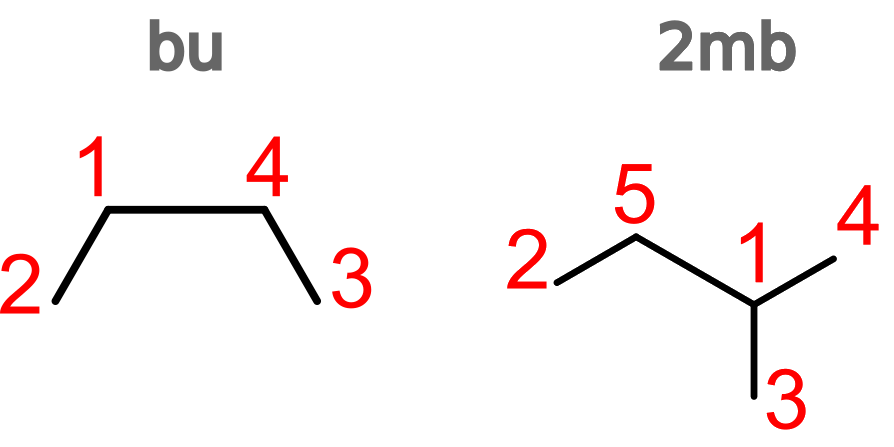
\includegraphics[width=.3\textwidth]{alkane-structures}
  \caption{Structures and atom indexing of the butane (\texttt{bu})
    and 2-methylbutane (\texttt{2mb}) molecules.}
  \label{fig:alkane-structures}
\end{figure}

\section{File Structure}
\label{sec:tutorial-file-structure}

The tutorial files can be found inside the \texttt{examples}
directory, which is organized as follows:

\begin{lstlisting}
|--- coords
|   |--- 2mb.g96
|   |--- bu.g96
|--- inp
|   |--- all-terms.inp
|   |--- custom-terms.inp
|--- qm
|   |--- 2mb.dat
|   |--- bu.dat
|--- stp
|   |--- 2mb_atomic.stp
|   |--- 2mb_pairs.stp
|   |--- bu_atomic.stp
|   |--- bu_pairs.stp
|--- wei
    |--- 2mb.dat
    |--- bu.dat
\end{lstlisting}
\vspace{1ex}\par

\noindent The contents of the directories above are:
\begin{itemize}
\item [---] \texttt{coords}: Initial coordinates of the systems (a single conformation each).
\item [---] \texttt{inp}: INP files with the input variables for the \profileropt{} runs. 
\item [---] \texttt{qm}: Quantum-mechanical reference data of the systems.
\item [---] \texttt{stp}: STP files with topology, reference dihedral and optimization targets of each system.
\item [---] \texttt{wei}: User-specified weight files.
\end{itemize}
%
Note that there are two INP files in the \texttt{inp} directory: one
for the optimization involving dihedral terms of all multiplicities
(\texttt{all-terms.inp}) and one for a single multiplicity
(\texttt{custom-terms.inp}).
%
There are also two STP files for each system in the \texttt{stp}
directory: one for the optimization of the CH3-CH3 pairtype
(\texttt{*\under{}pairs.stp}) and one for the CH3 atomtype
(\texttt{*\under{}atomic.stp}).
%
These files, and also the weight files in the \texttt{wei} directory,
will be discussed in more details in the following sections.

\section{Generating Torsional-Scan Trajectories}
\label{sec:tutorial-profilergen}

The first step in this tutorial is to generate torsional-scan
trajectories for the two systems.
%
These will serve as input trajectories to \profileropt{} later on in
the parameter optimization step.
%
To perform the torsional scans, only the coordinate and
STP files of each system are necessary.
%
The latter must contain the topology part and the
\texttt{[~refdihedral~]} block specifying the reference dihedral of
the scan (see \autoref{sec:file-formats-STP}).
%
For this tutorial, it is irrelevant which of the two STP files of each
system are chosen for performing its scan, since they are equivalent
in terms of their force-field parameters.
%
%
For example, the \texttt{stp/bu\under{}pairs.stp} file reads

\begin{lstlisting}[language=gromacs]
[ defaults ]
; nbfunc comb-rule gen-pairs fudgeLJ fudgeQQ
1        1         atomic    1.0     1.0

[ atoms ]
; type   c6                  c12                 cs6                 cs12                        q
CH2      7.4684160e-03       3.3965580e-05       4.7238130e-03       4.7419260e-06          0.0000
CH3      9.6138020e-03       2.6646240e-05       6.8525280e-03       6.0308650e-06          0.0000
CH3      9.6138020e-03       2.6646240e-05       6.8525280e-03       6.0308650e-06          0.0000
CH2      7.4684160e-03       3.3965580e-05       4.7238130e-03       4.7419260e-06          0.0000

[ nbpairs ]
;  ai   aj  type
    2    3    2     

[ bonds ]
;  ai   aj   type      l0          kb
    1    3    2      0.1530  7.1500e+06 
    1    4    2      0.1530  7.1500e+06 
    2    4    2      0.1530  7.1500e+06 

[ angles ]
;  ai   aj   ak   type   theta0      ka
    3    1    4    2    111.00    530.00 
    1    4    2    2    111.00    530.00 

[ dihedrals ]
;  ai   aj   ak   al   type      phi          k         mult
    3    1    4    2    1      0.0000      5.9200        3 

[ dihedrals ]
; improper dihedrals
;  ai   aj   ak   al   type      phi          k         

[ optpairs ]
; idxs
2   3   

[ optdihedrals ]
; idxs
3   1   4   2   

[ refdihedral ]
; idx
3   1   4   2
\end{lstlisting}\vspace{2ex}\par

\noindent 
%
and specifies that the torsional scan will be peformed along the
CH3-CH2-CH2-CH3 dihedral angle.
%
The optimization blocks \texttt{[~opt*~]} are not necessary to run
\profilergen{} and will be ignored in this step.

We now proceed to performing the torsional scans.
%
First, it is convenient to create new directories to receive the
\profilergen{} output files. Go inside the \texttt{examples} directory
and run the command:

\begin{lstlisting}
  mkdir scans scans/bu scans/2mb
\end{lstlisting}
\vspace{1ex}\par

\noindent to create them for each system.
%
Now, it is time to run \profilergen{}.
%
For butane, this can be done by running the command:\footnote{Backslashes are used to escape the newline character throughout the entire chapter.}

\begin{lstlisting}
../../profilerGen.py \
    -c coords/bu.g96 \
    -t stp/bu_pairs.stp \
    -dr 0 10 360 \
    -dk 5000 \
    -min 1 \
    -dx0 0.02 \
    -dxm 0.20 \
    -dele 1.0e-09 \
    -nsteps 500000 \
    -op scans/bu/bu
\end{lstlisting}\vspace{1ex}\par

\noindent To consult the meaning of each command-line option, see
\autoref{sec:program-gen}.
%
The command above performs a torsional scan of which the steps are
$0,10,20\ldots360$~deg.
%
At each step of the scan, the energy minimization is performed with a
steepest-descents algorithm until the (absolute) energy difference
between successive steps is less than $1.0\times 10^{-9}$
kJ~mol$^{-1}$ or until 500000 steps are carried out.
%
The resulting energy profile is reported in \texttt{scans/bu/bu.dat}
and is also plotted in \autoref{fig:tutorial-profiles}.
%
The torsional-scan trajectory is stored in \texttt{scans/bu/bu.xyz}.
%
For 2-methylbutane, we proceed in a similar way, replacing \texttt{bu}
with \texttt{2mb}:

\begin{lstlisting}
../../profilerGen.py \
    -c coords/2mb.g96 \
    -t stp/2mb_pairs.stp \
    -dr 0 10 360 \
    -dk 5000 \
    -min 1 \
    -dx0 0.02 \
    -dxm 0.20 \
    -dele 1.0e-09 \
    -nsteps 500000 \
    -op scans/2mb/2mb
\end{lstlisting}\vspace{1ex}\par

\noindent Once again, the resulting energy profile is reported in
\texttt{scans/2mb/2mb.dat} and is also plotted in
\autoref{fig:tutorial-profiles}.
%
The torsional-scan trajectory is stored in \texttt{scans/2mb/2mb.xyz}.
%

\section{Optimizing the Parameters}
\label{sec:tutorial-profileropt}

In the beginning of the chapter, four scenarios of parameter
optimization were listed.
%
Any given scenario differs from the other three only in the choice of
the STP and/or INP files and/or in the command-line options given to
\profileropt{}.
%
For this reason, we will discuss in details only the first of these
scenarios.
%
For the remaining ones, we will only point out the differences in the
corresponding input files or command-line options.
%

Bear in mind that, as the \profileropt{} code currently stands, each
run may take a couple of hours, even for the rather simple examples in
this tutorial.
%
For the sake of speed, you might want to consider parallelizing each
run, which can be done with the \texttt{-np} command-line option (see
\autoref{sec:program-opt}).
%
However, this leads to loss of reproducibility, which originates in
technical issues regarding random number generation when the
\texttt{multiprocessing} library is used for parallelization (as is
our case).
%
This is a limitation that we intend to address in future versions of
the program.
%
For this tutorial, we prioritize reproducibility instead of speed so
we report the commands without requesting parallelization.
%
Also, we supply the output files of the runs of each scenario in the
\texttt{examples\_results} directory.

\subsection{Scenario 1}
\label{sec:tutorial-scenario-1}

This scenario is defined by uniform weights, torsional terms of all
six multiplicities and pairtype optimization.
%
These settings are configured in the STP files
\texttt{stp/*\under{}pairs.stp} and the in the INP file
\texttt{inp/all-terms.inp}.
%
In the STP files, pairtype optimization is achieved by specifying the
Lennard-Jones optimization targets using the block
\texttt{[~optpairs~]}.
%
%
For example, in the STP file of 2-methylbutane
(\texttt{stp/2mb\under{}pairs.stp}), the fragment that reads

\begin{lstlisting}[language=gromacs]
[ optpairs ]
; idxs
2   3
2   4
\end{lstlisting}\vspace{1ex}\par

\noindent indicates that the two CH3-CH3 nonbonded pairs of which the
involved atoms are 2, 3 and 2, 4 are the targets of the Lennard-Jones
optimization. It is followed by the fragment
%

\begin{lstlisting}[language=gromacs]
[ optdihedrals ]
; idxs
4   1   5   2   
\end{lstlisting}\vspace{1ex}\par

\noindent that sets the dihedral angle CH3-CH1-CH2-CH3 formed by the
atoms 4, 1, 5 and 2 as the target of the torsional optimization.

The uniform weights and the funcional form of the torsional terms are
set in the INP file type.
%
The descriptions of all variables specified in this file are given in
\autoref{table:input-variables}, in which cross-references to the
meaning of their allowed values are also found.
%
For the sake of thoroughness, we will briefly comment the file that
corresponds to this scenario (\texttt{inp/all-terms.inp}), proceeding
block by block.

First, in

\begin{lstlisting}[language=gromacs]
[ parameter_optimization ]
; NTORS   NLJ   FTORS
      1     1       1    
; TORSNT[I]
; I=  1     2     3     4     5     6
      1     1     1     1     1     1
; LJNT[I]
; I=  1     2
;   CS6  CS12
      1     1
; WTEMP
      0
\end{lstlisting}\vspace{1ex}\par

\noindent the optimization of both torsional (NTORS) and
Lennard-Jones (NLJ) terms is set up.
%
For the former, a standard proper dihedral functional form (FTORS)
with terms of all six multiplicities (TORSNT) is used.
%
For the latter, both the attractive and the repulsive components are
optimized (LJNT).
%
Finally, if weight files are not supplied when \profileropt{} is
called, the fallback behavior is set to using uniform weights (WTEMP).

In

\begin{lstlisting}[language=gromacs]
[ seed ]
;   SEED
   19804
\end{lstlisting}\vspace{1ex}\par

\noindent the random number generator seed is set to 17135.
%
The control of the seed is useful for reproducibility purposes.
%
As long as parallelization is not requested, two \profileropt{} runs
with the same seed will yield the same results.

In

\begin{lstlisting}[language=gromacs]
[ parameter_randomization ]
;    PINV
       50
; DIST[I]  MIN[I]    MAX[I]     MEAN[I]  STDDEV[I]
; Torsional
        2       0        30        10.0        5.0 
; CS6
        2       0         1        8e-3      24e-3
; CS12
        2       0         1        8e-6      24e-6
\end{lstlisting}\vspace{1ex}\par

\noindent the details of the obtention of random parameters are set
up.
%
The distributions (DIST) from which torsional, $CS_6$ and $CS_{12}$
values are drawn, respectively, are specified along with their mean
(MEAN), standard deviation (STDDEV) and minimum (MIN) and maximum
allowed (MAX) values.
%
All of these distributions are LogNormal.
%
In the case of torsional parameters, after randomly obtained, they may
have their sign reversed with a probability of 0.50 (PINV).

In 

\begin{lstlisting}[language=gromacs]
[ genetic_algorithm ]
; POPSIZE    NGENS
      128     50
; SELTYPE     NTEL
        4        2
;  CRTYPE   CRRATE MUTRATE
        2      100      40
\end{lstlisting}\vspace{1ex}\par

\noindent the details of the genetic algorithm are set up.
%
The population size (POPSIZE) is set to 128, out of which 2 are elite
individuals (NTEL).
%
The tournament selection operator is chosen (SELTYPE), along with the
heuristic crossover operator (CRTYPE).
%
The crossover probability (CRRATE) is set to 1, \textit{i.e.} every
time two parents reproduce, there is crossover, while the mutation
probability (MUTRATE) is set to 0.4.
%
The genetic algorithm is configured to run for 50 generations (NGENS).

In

\begin{lstlisting}[language=gromacs]
[ writetraj ]
; NSTE   NSTP
     5      5
\end{lstlisting}\vspace{1ex}\par

\noindent the frequencies of writing individual energy profiles (NSTE)
and individual parameters (NSTP) to the TRE and TRP files are
specified.
%
In this case, these values are written to disk every 5 generations.

In

\begin{lstlisting}[language=gromacs]
[ minimization ]
; MALG[I]    DX0[I]  DXM[I]  NMAX[I]     DELE[I]
        1      0.02     0.2       20        1e-2
        1      0.02     0.2   500000        1e-9

\end{lstlisting}\vspace{1ex}\par

\noindent the minimization algorithm settings are specified.
%
They correspond to two steepest-descents algorithms (MALG) of
different precision (DELE) and duration (NMAX).
%
The first one refers to the routine minimization performed for every
individual; it runs for at most 20 steps or until the energy
difference between successive steps is less than 0.01 kJ~mol$^{-1}$.
%
The second one refers to the final minimization performed only for the
optimal individual; it runs for at most 500000 steps or until the energy
difference between successive steps is less than 10$^{-9}$
kJ~mol$^{-1}$.
%
The steepest-descents algorithm was chosen instead of the
conjugate-gradients one because it is more robust.
%
The conjugate-gradients algorithm may fail when the minimization is
performed on individuals with ``unbalanced'' parameter values, which
typically occur on the first generations or after a mutation.

In

\begin{lstlisting}[language=gromacs]
[ torsional_scan ]
;   RFRST  RSTEP  RLST   RFCT
        0     10   360   5000
\end{lstlisting}\vspace{1ex}\par

\noindent the torsional-scan details are specified.
%
The scan dihedral angles are set to $0,10,20\ldots 360$~deg and
maintained with a dihedral restraint of which the force constant is
5000 kJ~mol$^{-1}$~rad$^{-2}$.
%
It is important that these settings (except for the force constant)
match those of the input torsional-scan trajectories.
%
By comparing the contents of this block with the command-line options
of the \profilergen{} runs of \autoref{sec:tutorial-profilergen}, one
can easily see that this is the case.

With the input files explained, we proceed to the parameter
optimization.
%
First, it is once again convenient to create a directory for the
output files of \profileropt{}:

\begin{lstlisting}
mkdir scenario_1
\end{lstlisting}\vspace{1ex}\par

\noindent To perform the optimization, run the following command:

\begin{lstlisting}
../../profilerOpt.py \
    -r qm/bu.dat qm/2mb.dat \
    -c scans/bu/bu.xyz scans/2mb/2mb.xyz \
    -t stp/bu_pairs.stp stp/2mb_pairs.stp \
    -i inp/all-terms.inp \
    -op scenario_1/opt
\end{lstlisting}\vspace{1ex}\par

\noindent A complete description of the command-line options can be
found in \autoref{sec:program-opt}.
%
In the above, note that $(i)$ the input trajectories of \profileropt{}
are the output trajectories of \profilergen{}
(\autoref{sec:tutorial-profilergen});
%
$(ii)$ the input STP files are those for pairtype optimization
%
and $(iii)$ the input INP file is the one where a periodic dihedral
with all six multiplicities is specified.
%
During execution, \profileropt{} will notify in \texttt{stdout} the
start and completion of each generation.
%
It will also notify each time a new best individual is found,
informing the value of its weighted RMSD.
%

As indicated in \autoref{sec:program-opt}, a successful run of
\profileropt{} will create several output files of which the formats
are described in \autoref{sec:file-formats-file-formats}.
%
For the sake of thoroughness, we will comment on each of these output
files and the interpretation of their contents.
%
The TRR output file (\texttt{scenario\under{}1/opt.trr}) reads

\begin{lstlisting}
# GEN               AVG              BEST
    0     2.9678611e+02     1.4876041e+01
    1     9.2343584e+01     1.2555096e+01
...
   49     7.1041770e+01     2.3566693e+00
   50     2.4350660e+01     2.3566693e+00
\end{lstlisting}\vspace{1ex}\par

\noindent where the ellipsis \texttt{...} indicates the omission of
lines.
%
As indicated by the comments, the first column refers to the
generation (0 stands for the initial population), while the second and
last columns refer to the average and best (lowest) value of the
weighted RMSD, respectively, at the given generation.
%
This file is useful to inspect the diversity of individuals in the GA
and also their convergence along the generations.

The TRP output file (\texttt{scenario\under{}1/opt.trp}) reads

\begin{lstlisting}
1    
#   PHI1            K1   M1 ... PHI6            K6   M6               CS6              CS12             WRMSD
    0.00   -13.6573644    1 ... 0.00     7.8184962    6     1.1244283e-03     4.2265186e-06     1.2555096e+01
    0.00    -9.6352254    1 ... 0.00    -3.1527857    6     4.2770074e-03     2.4808228e-06     1.3642115e+01
...                         ...
    0.00    13.4845343    1 ... 0.00     6.4649437    6     7.1490046e-03     6.3541647e-09     1.7612964e+03
    0.00    12.2490638    1 ... 0.00     6.3990019    6     2.1167276e-02     2.1299433e-08     3.9020127e+03
6    
#   PHI1            K1   M1 ... PHI6            K6   M6               CS6              CS12             WRMSD
\end{lstlisting}\vspace{1ex}\par

\noindent where the ellipsis \texttt{...} indicates the omission of
lines and columns.
%
The fragment reproduced above reports the GA-individual parameters
(one individual per line) and the corresponding weighted RMSD of the
first generation, as indicated by the top number.
%
The meaning of each column is explained by the comments below the
generation number.
%
As indicated by the last lines, the data for the first generation is
followed by similarly structured data for the sixth generation (since
the frequency of writing to this file was set to five generations in
the input variable NSTP).
%

The TRE output files (\texttt{scenario\under{}1/opt\under{}1.tre} and
\texttt{scenario\under{}1/opt\under{}2.tre}) report the energy
profiles of all individuals for all generations.
%
There is one such file for each system, and they are numbered in the
same order in which the system files are supplied to \profileropt{}
(in this case, 1 refers to butane and 2 refers to 2-methylbutane).
%
For example, the butane TRE file reads

\begin{lstlisting}
1    
#    ANG              IND1 ...        IND128
    0.00     2.2426570e+01 ... 1.5073598e-01
   10.00     1.7133472e+01 ... 1.4272572e+01
...                        ...
  350.00     1.7133447e+01 ... 1.4374804e+01
  360.00     2.2428204e+01 ... 0.0000000e+00
6
#    ANG              IND1 ...        IND128  
\end{lstlisting}\vspace{1ex}\par

\noindent where the ellipsis \texttt{...} indicates the omission of lines and
columns.
%
The fragment reproduced above corresponds to the first generation of
the GA, as indicated by the top number.
%
The first column lists the angles of the torsional scan.
%
From the second column to the last, the corresponding energy profiles
of each individual are given, one per column.
%
As indicated by the last lines, the data for the first generation is
followed by similarly structured data for the sixth generation (since
the frequency of writing to this file was set to five generations in
the input variable NSTE).

The IFP output file (\texttt{scenario\under{}1/opt.ifp}) reads

\begin{lstlisting}
#              CS6              CS12
     2.2379720e-03     3.4437180e-06
#              PHI                 K    M
              0.00         0.6443053    1
              0.00         0.8438238    2
              0.00         6.7092465    3
              0.00        -0.7038652    4
              0.00         0.4910962    5
              0.00         0.5522696    6
#            WRMSD
     2.3566693e+00
\end{lstlisting}\vspace{1ex}\par

\noindent and reports the results of the parameter optimization: the
parameters of the optimal individual and the corresponding weighted
RMSD.
%
The data is clearly explained by the accompanying comments.


The torsional-scan trajectories of the optimal individual and the
corresponding energy profiles are written to the output files with XYZ
and DAT extensions, respectively.
%
These files are:

\begin{lstlisting}
scenario_1/opt_1.dat
scenario_1/opt_1.xyz
scenario_1/opt_2.dat
scenario_1/opt_2.xyz
scenario_1/opt_minim_1.dat
scenario_1/opt_minim_1.xyz
scenario_1/opt_minim_2.dat
scenario_1/opt_minim_2.xyz
\end{lstlisting}\vspace{1ex}\par
\noindent Each file is identified with the number of the system and
with a string indicating the minimization algorithm used in its
obtention.
%
The number of the system is defined by the order in which the system
files were given as input to \profileropt{}, like in the TRE files.
%
The minimization algorithm is identified with the ``\texttt{minim}''
string:
%
its presence indicates that the file corresponds to the enhanced
minimization algorithm settings, while
%
its absence indicates the less-precise minimization settings involved
in every generation of the GA.
%
The optimal energy profiles of
\texttt{scenario\under{}1/opt\under{}minim\under{}1.dat} and
\texttt{scenario\under{}1/opt\under{}minim\under{}2.dat} are plotted
in \autoref{fig:tutorial-profiles}.

\subsection{Scenario 2}
\label{sec:tutorial-scenario-2}

This scenario differs from Scenario 1 in the weights given to the
reference data.
%
Instead of using uniform weights, custom weights are supplied
\textit{via} the files \texttt{wei/bu.dat} and \texttt{wei/2mb.dat}.
%
In these files, data points that are close to peaks and valleys are
given weight 1, and the remaining ones are given weight 0,
\textit{i.e.}, they are irrelevant in the optimization (see
\autoref{fig:qm-and-wei}).
%
To perform the optimization, the most important change necessary is to
include the weight files in the call to \profileropt, \textit{i.e.},

\begin{lstlisting}
../../profilerOpt.py \
    -r qm/bu.dat qm/2mb.dat \
    -c scans/bu/bu.xyz scans/2mb/2mb.xyz \
    -t stp/bu_pairs.stp stp/2mb_pairs.stp \
    -i inp/all-terms.inp \
    -op scenario_2/opt \
    -w wei/bu.dat wei/2mb.dat
\end{lstlisting}\vspace{1ex}\par

\noindent where the last line contains the weight files.
%
In the above, it is assumed that a directory
\texttt{scenario\under{}2} has been previously created to store the
output files.
%
After the run is finished, the optimal parameters reported in the IFP
file are

\begin{lstlisting}
#              CS6              CS12
     2.9068136e-03     2.9907985e-06
#              PHI                 K    M
              0.00        -0.2056776    1
              0.00         0.1713483    2
              0.00         6.6991703    3
              0.00        -0.0621579    4
              0.00         1.5542293    5
              0.00         1.3870725    6
#            WRMSD
     1.1921891e+00
\end{lstlisting}\vspace{1ex}\par

\noindent The corresponding energy profiles of
\texttt{scenario\under{}2/opt\under{}minim\under{}1.dat} and
\texttt{scenario\under{}2/opt\under{}minim\under{}2.dat} are plotted
in \autoref{fig:tutorial-profiles}.

\begin{figure}[tb]
  \centering
  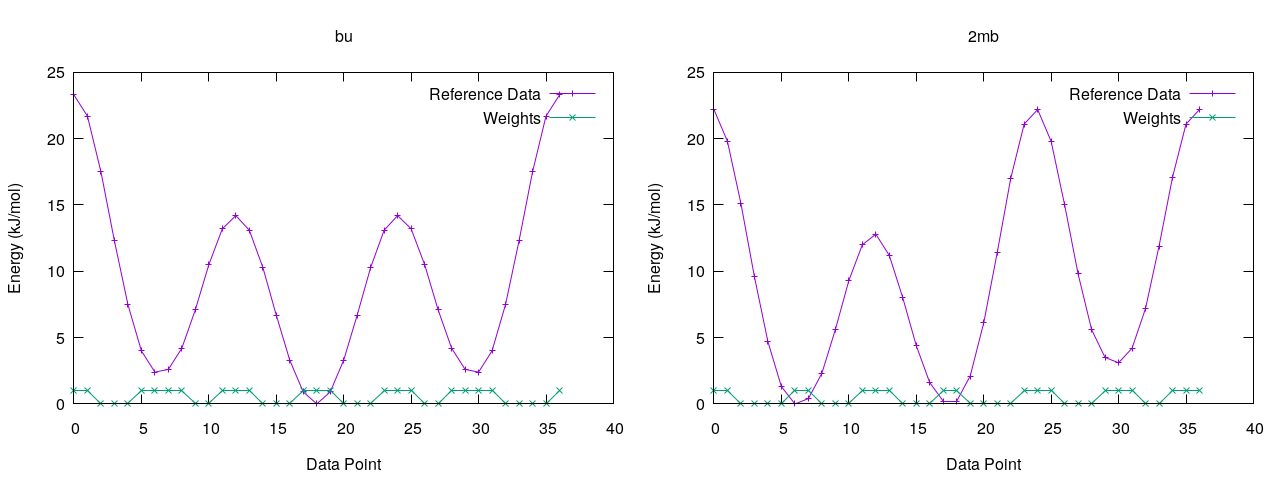
\includegraphics[width=\textwidth]{qm-and-weis}
  \caption{Reference data of the optimization and custom weights for
    each system. The $y$-axis labels refer only to the reference data;
    the weights are dimensionless.}
  \label{fig:qm-and-wei}
\end{figure}

\subsection{Scenario 3}
\label{sec:tutorial-scenario-3}

This scenario differs from Scenario 1 in the functional form of the
torsional terms.
%
Instead of all summands in \autoref{eq:proper-standard-energy}, only
the term with multiplicity equal to 3 is optimized, while the others
are set to zero.
%
This can be achieved by altering the value of the input variable
TORSNT in the block \texttt{[~parameter\under{}optimization~]} of the
INP file.
%
This is done in the \texttt{inp/custom-terms.inp} file, where this
block reads:

\begin{lstlisting}[language=gromacs]
[ parameter_optimization ]
; NTORS   NLJ   FTORS
      1     1       1    
; TORSNT[I]
; I=  1     2     3     4     5     6
      0     0     1     0     0     0
; LJNT[I]
; I=  1     2
;   CS6  CS12
      1     1
; WTEMP
      0
\end{lstlisting}\vspace{1ex}\par

\noindent 
%
To perform the optimization, the most important change necessary is to
use the appropriate INP file in the call to \profileropt,
\textit{i.e.},

\begin{lstlisting}
../../profilerOpt.py \
    -r qm/bu.dat qm/2mb.dat \
    -c scans/bu/bu.xyz scans/2mb/2mb.xyz \
    -t stp/bu_pairs.stp stp/2mb_pairs.stp \
    -i inp/custom-terms.inp \
    -op scenario_3/opt 
\end{lstlisting}\vspace{1ex}\par

\noindent In the above, it is assumed that a directory
\texttt{scenario\under{}3} has been previously created to store the
output files.
%
After the run is finished, the optimal parameters reported in the IFP
file are

\begin{lstlisting}
#              CS6              CS12
     2.9293877e-03     2.9476463e-06
#              PHI                 K    M
              0.00         0.0000000    1
              0.00         0.0000000    2
              0.00         7.2805242    3
              0.00         0.0000000    4
              0.00         0.0000000    5
              0.00         0.0000000    6
#            WRMSD
     6.5948745e-01
\end{lstlisting}\vspace{1ex}\par

\noindent The corresponding energy profiles of
\texttt{scenario\under{}3/opt\under{}minim\under{}1.dat} and
\texttt{scenario\under{}3/opt\under{}minim\under{}2.dat} are plotted
in \autoref{fig:tutorial-profiles}.

\subsection{Scenario 4}
\label{sec:tutorial-scenario-4}

This scenario differs from Scenario 1 in the way that the target of
the Lennard-Jones optimization is specified.
%
Instead of the CH3--CH3 pairtype, the CH3 atomtype is targeted in the
optimization.
%
Note that these approaches are equivalent for the two molecules
considered in this tutorial, since the only 1--4 nonbonded pairtype
that they contain is the CH3--CH3 one.
%
If there were any other 1--4 nonbonded pairs involving CH3, this would
not be the case, because the atomtype optimization would also affect
them, while the pairtype optimization would not.
%

Atomtype optimization can be achieved by listing the target atoms in
the \texttt{[~optatoms~]} block of the STP files, which replaces the
\texttt{[~optpairs~]} block of the previous scenarios.
%
This is done in the STP files \texttt{stp/bu\under{}atomic.stp} and
\texttt{stp/2mb\under{}atomic.stp}.
%
For example, in the 2-methylbutane STP file,

\begin{lstlisting}[language=gromacs]
[ optatoms ]
; idxs
2   3   4
\end{lstlisting}\vspace{1ex}\par

\noindent indicates that the atoms 2, 3 and 4 receive the
Lennard-Jones parameters of the optimal GA individual.
%
To perform the optimization, the most important change necessary is to
use the appropriate STP files in the call to \profileropt,
\textit{i.e.},

\begin{lstlisting}
../../profilerOpt.py \
    -r qm/bu.dat qm/2mb.dat \
    -c scans/bu/bu.xyz scans/2mb/2mb.xyz \
    -t stp/bu_atomic.stp stp/2mb_atomic.stp \
    -i inp/all-terms.inp \
    -op scenario_4/opt
\end{lstlisting}\vspace{1ex}\par

\noindent In the above, it is assumed that a directory
\texttt{scenario\under{}4} has been previously created to store the
output files.
%
After the run is finished, the optimal parameters reported in the IFP
file are:

\begin{lstlisting}
#              CS6              CS12
     2.2379720e-03     3.4437180e-06
#              PHI                 K    M
              0.00         0.6443053    1
              0.00         0.8438238    2
              0.00         6.7092465    3
              0.00        -0.7038652    4
              0.00         0.4910962    5
              0.00         0.5522696    6
#            WRMSD
     2.3566693e+00
\end{lstlisting}\vspace{1ex}\par

\noindent Note that they are identical to the ones obtained in
Scenario 1 (\autoref{sec:tutorial-scenario-1}), as anticipated above.
%
The corresponding energy profiles of
\texttt{scenario\under{}4/opt\under{}minim\under{}1.dat} and
\texttt{scenario\under{}4/opt\under{}minim\under{}2.dat} are plotted
in \autoref{fig:tutorial-profiles}.

\begin{figure}[tb]
  \centering
  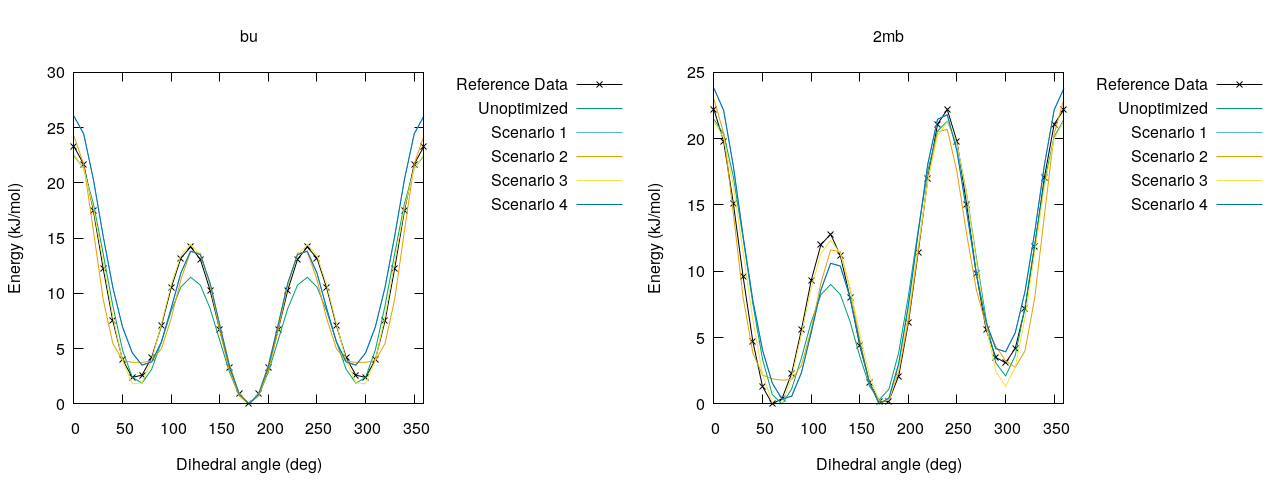
\includegraphics[width=\textwidth]{tutorial-profiles}
  \caption{Optimal energy profiles of the four scenarios studied in
    this tutorial, along with the reference and unoptimized data for
    each system.  Note that the lines of Scenario 1 and Scenario 4
    superimpose over each other.  The unoptimized data is from the
    energy profiles obtained with \profilergen{} in
    \autoref{sec:tutorial-profilergen}, using the original parameters
    of the STP files.}
  \label{fig:tutorial-profiles}
\end{figure}

\begin{thebibliography}{9}
\bibitem{GROMOS-doc} van Gunsteren, W. F., Billeter, S. R., Eising,
  A. A., Hünenberger, P. H., Krüger, P., Mark, A. E., Scott,
  W. R. P. and Tironi, I. G. Biomolecular Simulation: The GROMOS96
  Manual and User Guide. Volume~2:~Algorithms and Formulae for
  Modelling of Molecular Systems, Vdf Hochschulverlag AG an der ETH
  Zürich, Zürich, Switzerland, 1996.
\bibitem{GROMACS-doc} Abraham, M.~J., van~der~Spoel, D., Lindahl,~E.,
  Hess,~B. and the GROMACS development team. GROMACS User Manual
  version 2019. \url{http://www.gromacs.org}.
\end{thebibliography}

\appendix
\chapter{MIT License}
\label{appendix:MIT-license}

\begin{verbatim}
MIT License

Copyright (c) 2020 mssm-labmmol

Permission is hereby granted, free of charge, to any person obtaining a copy
of this software and associated documentation files (the "Software"), to deal
in the Software without restriction, including without limitation the rights
to use, copy, modify, merge, publish, distribute, sublicense, and/or sell
copies of the Software, and to permit persons to whom the Software is
furnished to do so, subject to the following conditions:

The above copyright notice and this permission notice shall be included in all
copies or substantial portions of the Software.

THE SOFTWARE IS PROVIDED "AS IS", WITHOUT WARRANTY OF ANY KIND, EXPRESS OR
IMPLIED, INCLUDING BUT NOT LIMITED TO THE WARRANTIES OF MERCHANTABILITY,
FITNESS FOR A PARTICULAR PURPOSE AND NONINFRINGEMENT. IN NO EVENT SHALL THE
AUTHORS OR COPYRIGHT HOLDERS BE LIABLE FOR ANY CLAIM, DAMAGES OR OTHER
LIABILITY, WHETHER IN AN ACTION OF CONTRACT, TORT OR OTHERWISE, ARISING FROM,
OUT OF OR IN CONNECTION WITH THE SOFTWARE OR THE USE OR OTHER DEALINGS IN THE
SOFTWARE.
\end{verbatim}

\end{document}